\documentclass[a4paper, UKenglish, cleveref, autoref, thm-restate, colorlinks]{lipics-v2021}

\usepackage{amsmath}
\usepackage{amssymb}
\usepackage{color}
\usepackage{prooftree}
\usepackage{stackrel}
\usepackage{tikz}

\newcommand{\todo}[1]{}
\renewcommand{\todo}[1]{{\color{red} TODO: {#1}}}

\usetikzlibrary{patterns}

\bibliographystyle{plainurl}

\newcommand{\eps}[1]{\epsilon{#1}.}
\newcommand{\fall}[1]{\forall{#1}.}
\newcommand{\lam}[1]{\lambda{#1}.}
\newcommand{\xsts}[1]{\exists{#1}.}

\title{All watched over by machines of loving grace}
\titlerunning{Supervisionary system description}

\begin{CCSXML}
<ccs2012>
   <concept>
       <concept_id>10003752.10003790.10003800</concept_id>
       <concept_desc>Theory of computation~Higher order logic</concept_desc>
       <concept_significance>300</concept_significance>
       </concept>
   <concept>
       <concept_id>10003752.10003790.10003794</concept_id>
       <concept_desc>Theory of computation~Automated reasoning</concept_desc>
       <concept_significance>500</concept_significance>
       </concept>
   <concept>
       <concept_id>10003752.10003790.10002990</concept_id>
       <concept_desc>Theory of computation~Logic and verification</concept_desc>
       <concept_significance>500</concept_significance>
       </concept>
   <concept>
       <concept_id>10011007.10010940.10010941.10010949</concept_id>
       <concept_desc>Software and its engineering~Operating systems</concept_desc>
       <concept_significance>300</concept_significance>
       </concept>
 </ccs2012>
\end{CCSXML}

\ccsdesc[300]{Theory of computation~Higher order logic}
\ccsdesc[500]{Theory of computation~Automated reasoning}
\ccsdesc[500]{Theory of computation~Logic and verification}
\ccsdesc[300]{Software and its engineering~Operating systems}

\keywords{Proof assistant design, operating systems, HOL, LCF, Supervisionary, system description, capabilities}

\author{Dominic P. Mulligan}{Automated Reasoning Group, Amazon Web Services, Cambridge, United Kingdom\footnote{All work done whilst employed within the Systems Research Group, Arm Research, Cambridge} \and \url{www.dominic-mulligan.co.uk}}{dominic.p.mulligan@gmail.com}{}{}
\authorrunning{Dominic P. Mulligan}

\Copyright{Dominic P. Mulligan}

\acknowledgements{We would like to thank Nick Spinale for many insightful conversations regarding Supervisionary, and Nathan Chong for helpful comments on an early draft of this paper.}

\begin{document}

\maketitle

\begin{abstract}
Modern operating systems are typically built around a trusted system component called the \emph{kernel} which amongst other things is charged with enforcing system-wide security policies.
Crucially, this component must be kept isolated from untrusted software at all times, which is facilitated by exploiting machine-oriented notions of separation: private memories, privilege levels, and similar.

Modern proof-assistants are typically built around a trusted system component called the \emph{kernel} which is charged with enforcing system-wide soundness.
Crucially, this component must be kept isolated from untrusted automation at all times, which is facilitated by exploiting programming-language notions of separation: module-private data structures, type-abstraction, and similar.

Whilst markedly different in purpose, in some essential ways operating system and proof-assistant kernels are tasked with the same job, namely enforcing system-wide invariants in the face of unbridled interaction with untrusted code.  Yet the mechanisms through which the two types of kernel protect themselves are significantly different.
In this paper, we introduce \emph{Supervisionary}, the kernel of a prototype programmable proof-checking system for Gordon's HOL that is organised in a manner more reminiscent of operating systems than typical LCF-style proof-checkers.
Supervisionary implements a kernel that executes at a relative level of privilege compared to untrusted automation, with trusted and untrusted system components communicating across a limited system call boundary.
Kernel objects, managed on behalf of user-space by the Supervisionary kernel, are referenced by handles which are passed back-and-forth by Supervisionary's system calls.

Unusually, Supervisionary has no ``metalanguage'' in the LCF sense, as the language used to implement the kernel, and the language used to implement automation, need not be the same.
\emph{Any} programming language can be used to implement automation for Supervisionary, providing the resulting binary respects the Supervisionary kernel calling convention and binary interface, with no risk to system soundness.
Further, we observe that Supervisionary allows arbitrary programming languages to be endowed with facilities for proof-checking.
Indeed, the handles that Supervisionary uses to reference kernel objects under its management may be thought of as a form of \emph{capability}, in the computer security sense.
Moreover, these capabilities are extremely expressive, essentially capturing the full expressive power of HOL, and can potentially be used to enforce fine-grained correctness and security properties of programs at runtime.
\end{abstract}

\section{Introduction}
\label{sect.introduction}

This paper studies the intersection of operating system design and implementations of the foundations of mathematics.
Research into the confluence of these two topics is, admittedly, a rather moribund affair at the moment.
Nevertheless, with this paper we hope to convince the reader that probing the intersection of these two areas is potentially very interesting by introducing \emph{Supervisionary}, a programmable proof-checking system for Gordon's HOL.
This system has a novel system design, with some interesting properties, and moreover some interesting consequences.
First, however, we begin with a scene-setting overview of common principles in operating system design and implementation.

\subsection{On operating systems}

\begin{figure}
\tikzset{every picture/.style={line width=0.75pt}} %set default line width to 0.75pt        
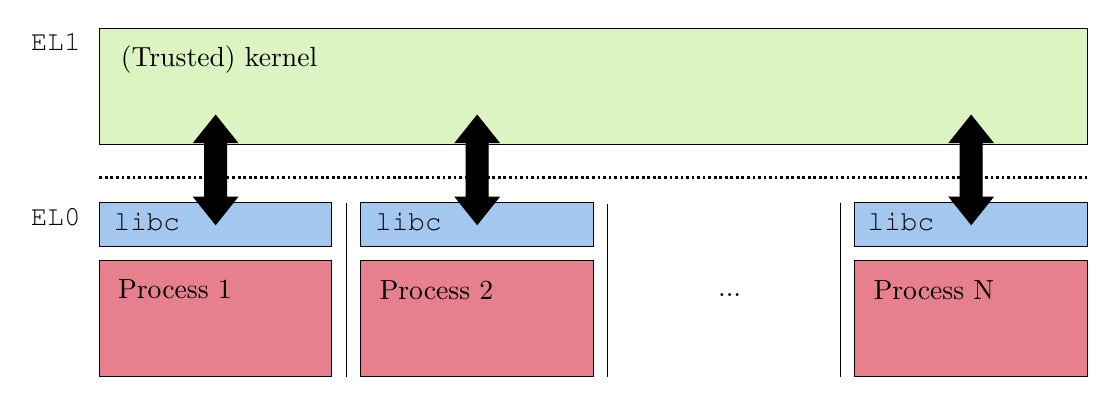
\begin{tikzpicture}[x=0.75pt,y=0.75pt,yscale=-0.7,xscale=0.7]
%uncomment if require: \path (0,300); %set diagram left start at 0, and has height of 300

%Straight Lines [id:da0238858095373361] 
\draw [line width=1]  [dash pattern={on 1pt off 1pt}]  (10,133) -- (690,133) ;
%Shape: Rectangle [id:dp18633003951104476] 
\draw  [fill={rgb, 255:red, 184; green, 233; blue, 134 }  ,fill opacity=0.5 ] (10,30) -- (690,30) -- (690,110) -- (10,110) -- cycle ;
%Straight Lines [id:da8836005156472156] 
\draw    (180,150) -- (180,270) ;
%Straight Lines [id:da0871105771687758] 
\draw    (360,151) -- (360,270) ;
%Straight Lines [id:da47486673087950704] 
\draw    (520,150) -- (520,270) ;
%Flowchart: Process [id:dp5014112861074582] 
\draw  [fill={rgb, 255:red, 208; green, 2; blue, 27 }  ,fill opacity=0.5 ] (10,190) -- (170,190) -- (170,270) -- (10,270) -- cycle ;
%Flowchart: Process [id:dp5474401833590941] 
\draw  [fill={rgb, 255:red, 208; green, 2; blue, 27 }  ,fill opacity=0.5 ] (190,190) -- (350,190) -- (350,270) -- (190,270) -- cycle ;
%Flowchart: Process [id:dp05943677937308278] 
\draw  [fill={rgb, 255:red, 208; green, 2; blue, 27 }  ,fill opacity=0.5 ] (530,190) -- (690,190) -- (690,270) -- (530,270) -- cycle ;
%Flowchart: Process [id:dp22719106375428721] 
\draw  [fill={rgb, 255:red, 74; green, 144; blue, 226 }  ,fill opacity=0.5 ] (10,150) -- (170,150) -- (170,180) -- (10,180) -- cycle ;
%Flowchart: Process [id:dp418634561741007] 
\draw  [fill={rgb, 255:red, 74; green, 144; blue, 226 }  ,fill opacity=0.5 ] (190,150) -- (350,150) -- (350,180) -- (190,180) -- cycle ;
%Flowchart: Process [id:dp5808126324898445] 
\draw  [fill={rgb, 255:red, 74; green, 144; blue, 226 }  ,fill opacity=0.5 ] (530,150) -- (690,150) -- (690,180) -- (530,180) -- cycle ;
%Left Right Arrow [id:dp18252152506193997] 
\draw  [fill={rgb, 255:red, 0; green, 0; blue, 0 }  ,fill opacity=1 ] (90,90) -- (105,108.75) -- (97.5,108.75) -- (97.5,146.25) -- (105,146.25) -- (90,165) -- (75,146.25) -- (82.5,146.25) -- (82.5,108.75) -- (75,108.75) -- cycle ;
%Left Right Arrow [id:dp937447124008122] 
\draw  [fill={rgb, 255:red, 0; green, 0; blue, 0 }  ,fill opacity=1 ] (270,90) -- (285,108.75) -- (277.5,108.75) -- (277.5,146.25) -- (285,146.25) -- (270,165) -- (255,146.25) -- (262.5,146.25) -- (262.5,108.75) -- (255,108.75) -- cycle ;
%Left Right Arrow [id:dp43564214029042536] 
\draw  [fill={rgb, 255:red, 0; green, 0; blue, 0 }  ,fill opacity=1 ] (610,90) -- (625,108.75) -- (617.5,108.75) -- (617.5,146.25) -- (625,146.25) -- (610,165) -- (595,146.25) -- (602.5,146.25) -- (602.5,108.75) -- (595,108.75) -- cycle ;

% Text Node
\draw (23,40) node [anchor=north west][inner sep=0.75pt]   [align=left] {{\fontfamily{rm}\selectfont (Trusted) kernel}};
% Text Node
\draw (434,211) node [anchor=north west][inner sep=0.75pt]   [align=left] {{\fontfamily{rm}\selectfont ...}};
% Text Node
\draw (18,155) node [anchor=north west][inner sep=0.75pt]   [align=left] {{\fontfamily{pcr}\selectfont libc}};
% Text Node
\draw (198,155) node [anchor=north west][inner sep=0.75pt]   [align=left] {{\fontfamily{pcr}\selectfont libc}};
% Text Node
\draw (537,155) node [anchor=north west][inner sep=0.75pt]   [align=left] {{\fontfamily{pcr}\selectfont libc}};
% Text Node
\draw (21,201) node [anchor=north west][inner sep=0.75pt]   [align=left] {{\fontfamily{rm}\selectfont Process 1}};
% Text Node
\draw (201,202) node [anchor=north west][inner sep=0.75pt]   [align=left] {{\fontfamily{rm}\selectfont Process 2}};
% Text Node
\draw (541,202) node [anchor=north west][inner sep=0.75pt]   [align=left] {{\fontfamily{rm}\selectfont Process N}};
% Text Node
\draw (-39,32) node [anchor=north west][inner sep=0.75pt]   [align=left] {{\fontfamily{pcr}\selectfont EL1}};
% Text Node
\draw (-39,152) node [anchor=north west][inner sep=0.75pt]   [align=left] {{\fontfamily{pcr}\selectfont EL0}};
\end{tikzpicture}
\caption{A schematic of the typical system organization of a commodity operating system and its associated user-space.
The kernel (in green) executes at a relative level of privilege, enforced by hardware, compared to processes executing in user-space (red)---we follow the Arm convention and show the kernel executing at \texttt{EL1} and user-space at \texttt{EL0}.
The two communicate across a system call boundary (dashed line) using system calls (black arrows).
User-space programs are typically written making use of an abstraction library, such as \texttt{libc} (blue), to abstract over this kernel interface.}
\label{fig.operating-system.schematic}
\end{figure}

Most commodity operating systems---that is, Microsoft Windows and Unix-derivatives\footnote{\emph{Commodity} here is used to guard against pedantic quibbling over research operating system designs---like exokernels~\cite{engler95exokernel} and other oddities---which arguably do not fit this pattern.}---fit a common pattern and are architected around a relatively self-contained, trusted component typically called the system \emph{kernel}~\cite{DBLP:books/daglib/0019512}.

The kernel is the sole component that can interface unfettered with all system resources, including devices and other system hardware.
Untrusted user-space applications make use of kernel interfaces in order to make use of a device or any other system resource managed by the kernel.
As a result, the kernel is essentially a ``pinch point'' for gating access to system resources.
The kernel also introduces a process abstraction in user-space and is responsible for ensuring the confidentiality and integrity of concurrently-executing processes, each of which are mutually mistrusting.
The kernel is therefore \emph{the} key component responsible for enforcing system-wide security policies, and essentially forms the ``root of all trust'' within a computing system.
It is therefore imperative that the kernel is itself isolated sufficiently from user-space software at all times, lest this role be undermined by a malefactor.

The kernel self-isolates by co-operating with its host hardware.
In support of this, mainstream microprocessors have, over the years, accreted a variety of now-familiar security features that an operating system kernel can use to defend itself from prying or interference.
These include \emph{exception levels} or \emph{privilege rings}, as they are variously called depending on the instruction set architecture, which introduce a notion of \emph{privilege} into the system.
Here, software executing at higher-privilege---in our case, an operating system kernel\footnote{Note that \emph{Cloud hosting} as a viable business proposition essentially rests on this trick being repeated again, with a hypervisor sat in a position of privilege compared to an operating system kernel---executing out of an even higher exception level---and enforcing separation betwixt operating system instances.}---gains permission to program sensitive system registers, adjust hardware operating frequencies and voltages, and generally control how the system operates.
Moreover, software executing at a higher-level of privilege can ``peer in'' and potentially modify the runtime state of software executing at a relatively lower-level of privilege, reading data from, or writing data to, a buffer within the memory space of an untrusted user-space process, for example.

Modern microprocessors also provide a form of memory management built around page tables (see e.g.~\cite{arm-vmsa}).
These data structures have a dual role: primarily, they are used for the virtualisation of system memory via address translation, granting user-space software the illusion that it owns the entire physical address space of the machine, presenting a virtual address space to user-space programs.
This process induces a notion of ownership of pages of physical memory within the system, with a page of physical memory ``owned'' by a principal---either the operating system, a user-space process, or both---if it is \emph{mapped in} to that principal's address space.
Moreover, page tables are also used for storing the attributes of pages of memory, including read-write-execute permissions.
By correctly initialising and managing these tables the kernel is able to keep its own code and data structures isolated---in a kernel-private memory area---that only it can access, safe from prying or interference by untrusted user-space.
As a result, for systems software on modern machines, isolation is enforced by a mix of low-level machine mechanisms: separate address spaces, private memory regions, and machine-enforced privilege checks on executing software.

To make itself useful, the kernel exposes a limited interface, used by user-space to request intercession by the kernel on its behalf---for example by granting user-space access to some device, the filesystem, a socket, or some other system resource under kernel management.
Dealing in generalities, to do this, the kernel exposes a suite of largely synchronous \emph{system calls} which can be invoked by user-space programs with dedicated machine instructions provided by the microprocessor---see Figure~\ref{fig.operating-system.schematic} for a diagrammatic schematic, for example.
On Arm platforms, with which the author is most familiar, these instructions induce a processor exception, forcing a \emph{context switch} which flips the flow of control into the kernel's system call handler, before eventually returning the flow of control back to the calling user-space program.
From user-space's point-of-view, system calls therefore have the appearance and effect of very CISC-like machine instructions, with the operating system kernel essentially presenting itself to user-space as \emph{silicon by other means}, extending the user-space fragment of the instruction set architecture of the microprocessor with new instructions.

Note that for this two-way dance to work, user-space and the kernel must work together by adopting a series of joint conventions.
These include a \emph{calling convention} describing how arguments and results are passed back-and-forth across the system call interface, and a \emph{binary interface} detailing how system calls are identified, how errors are reported back to user-space, and other miscellanea.\footnote{For more detail on the role of the system ABI, its other aspects, and its very real effects on the semantics of executing programs, see this~\cite{DBLP:conf/oopsla/KellMS16} outrageously well-written yet criminally under-cited overview.}
To help programmers adhere to these conventions, the operating system typically provides an abstraction layer to user-space, which on Unix variants typically takes the form of the system's C library, \texttt{libc}.
Note that this is generally just a convenience, and user-space software can always invoke system calls directly if wanted by invoking the correct machine instruction and adhering to the appropriate calling convention.\footnote{This is the case on Linux, though does not hold universally on all Unix derivatives.  For example Apple's MacOS and some BSD Unix variants generally consider the programming interface of the system C library as the interface of the kernel, proper, in some cases preventing any user-space code other than the system's \texttt{libc} library from invoking system calls directly, as a security mechanism.}

However, crucially, it is \emph{generally} not the case that the operating system kernel and untrusted user-space applications must be written in the same programming language for this all to work.
In particular, whilst most operating system kernels are written in C, or a C-language derivative, user-space programs can be written in a variety of languages, and are also commonly composed of multiple libraries, written in different programming languages, linked together.
Despite this, all are able to make use of system resources exposed by the kernel's system call interface by ensuring that they adhere to the calling convention and binary interface expected by the kernel.
In this respect, for commodity operating systems, the C-language may have prominence as a favoured language of system implementation, but by-and-large it is not \emph{special} or given an unduly prominent status by the kernel itself.

\subsection{On programmable proof-checkers}

\begin{figure}
\tikzset{every picture/.style={line width=0.75pt}} %set default line width to 0.75pt        
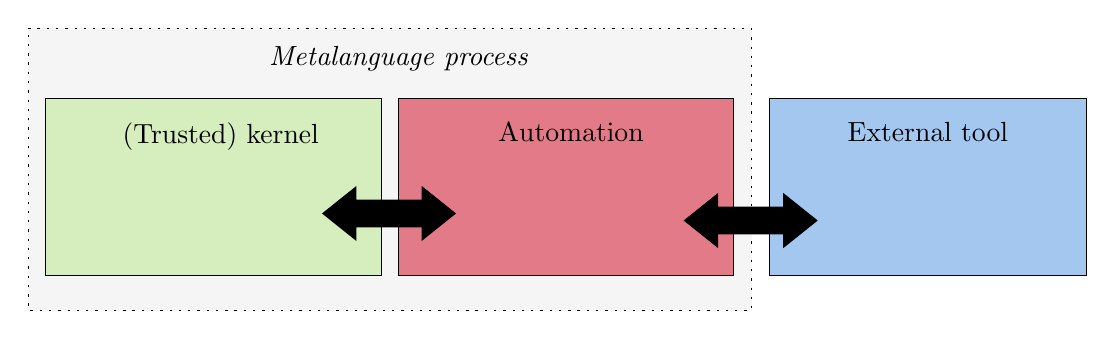
\begin{tikzpicture}[x=0.75pt,y=0.75pt,yscale=-0.85,xscale=0.85]
%uncomment if require: \path (0,300); %set diagram left start at 0, and has height of 300

%Shape: Rectangle [id:dp5145169571980753] 
\draw  [fill={rgb, 255:red, 155; green, 155; blue, 155 }  ,fill opacity=0.1 ][dash pattern={on 0.84pt off 2.51pt}] (10,10) -- (420,10) -- (420,170) -- (10,170) -- cycle ;
%Shape: Rectangle [id:dp7336028259076729] 
\draw  [fill={rgb, 255:red, 184; green, 233; blue, 134 }  ,fill opacity=0.5 ] (20,50) -- (210,50) -- (210,150) -- (20,150) -- cycle ;
%Shape: Rectangle [id:dp32707998554431983] 
\draw  [fill={rgb, 255:red, 208; green, 2; blue, 27 }  ,fill opacity=0.5 ] (220,50) -- (410,50) -- (410,150) -- (220,150) -- cycle ;
%Shape: Rectangle [id:dp3433596839522859] 
\draw  [fill={rgb, 255:red, 74; green, 144; blue, 226 }  ,fill opacity=0.5 ] (430,50) -- (610,50) -- (610,150) -- (430,150) -- cycle ;
%Left Right Arrow [id:dp2058390242799486] 
\draw  [fill={rgb, 255:red, 0; green, 0; blue, 0 }  ,fill opacity=1 ] (177,115) -- (195.75,100) -- (195.75,107.5) -- (233.25,107.5) -- (233.25,100) -- (252,115) -- (233.25,130) -- (233.25,122.5) -- (195.75,122.5) -- (195.75,130) -- cycle ;
%Left Right Arrow [id:dp5651724135135525] 
\draw  [fill={rgb, 255:red, 0; green, 0; blue, 0 }  ,fill opacity=1 ] (382,119) -- (400.75,104) -- (400.75,111.5) -- (438.25,111.5) -- (438.25,104) -- (457,119) -- (438.25,134) -- (438.25,126.5) -- (400.75,126.5) -- (400.75,134) -- cycle ;

% Text Node
\draw (145,19) node [anchor=north west][inner sep=0.75pt]   [align=left] {{\fontfamily{rm}\selectfont {\it Metalanguage process}}};
% Text Node
\draw (62,62) node [anchor=north west][inner sep=0.75pt]   [align=left] {{\fontfamily{rm}\selectfont (Trusted) kernel}};
% Text Node
\draw (275,62) node [anchor=north west][inner sep=0.75pt]   [align=left] {{\fontfamily{rm}\selectfont Automation}};
% Text Node
\draw (473,62) node [anchor=north west][inner sep=0.75pt]   [align=left] {{\fontfamily{rm}\selectfont External tool}};
\end{tikzpicture}
\caption{A schematic of the system organisation of a typical LCF-style proof assistant.
The trusted kernel (green) is linked against untrusted automation (red) existing within the same metalanguage process (dotted line) and communicate with each other using the kernel's API (leftmost black arrow).
External tools existing as separate processes (blue), must communicate with a shim layer written in the proof assistant's metalanguage to access the kernel (rightmost black arrow).}
\label{fig.proof-assistant.organization}
\end{figure}

Most modern proof-assistants---for example, systems in the wider HOL family~\cite{10.1007/s00165-019-00492-1, DBLP:conf/tphol/Harrison09a, DBLP:conf/tphol/SlindN08}, Coq~\cite{DBLP:conf/popl/HuetH14}, Matita~\cite{DBLP:conf/cade/AspertiRCT11}, NuPRL~\cite{DBLP:conf/cade/AllenCEKL00}, and similar---fit a common pattern and are architected around a relatively self-contained, trusted component typically called the system \emph{kernel}.

The system kernel is the sole component that can authenticate claims as legitimate theorems of the implemented logic.
Untrusted automation, residing outside of the kernel, must ``drive'' the kernel to derive a theorem on its behalf.
The kernel is therefore \emph{the} component responsible for ensuring system-wide soundness, and represents the ``root of all trust'' within the system.
It is therefore imperative that the kernel is able to isolate itself sufficiently from untrusted automation at all times.
This kernel-centric method of system organisation is known as \emph{the LCF approach} after Milner's eponymous system~\cite{DBLP:books/sp/Gordon79} which first introduced it, and is now the most common way of organising proof-checking systems today.
See Figure~\ref{fig.proof-assistant.organization} for a diagrammatic representation.

Most modern proof-assistants tend to be written in a \emph{metalanguage} which serves as the implementation language for both the kernel and the majority of the untrusted automation that modern proof-assistants provide to users.
This metalanguage is typically a strongly-typed functional programming language, for example an ML derivative such as OCaml or SML~\cite{DBLP:books/daglib/0069232}, and which offers strong modularity and abstraction features.
The kernel exploits these programming language features to hide its own data structures from untrusted automation and moreover exposes a carefully limited API for proof-construction and manipulation.
Notably, in an LCF-style system, the \emph{only} mechanism automation has for constructing an authenticated theorem is by using this API, with the inference rules of the logic exposed as a suite of \emph{smart constructors} manipulating an abstract type of theorems.
As a result, the kernel is therefore a ``pinch point'' for any proof-construction activity within the system.

Untrusted automation and the system kernel are linked together, and reside side-by-side in the same process when the proof-assistant is executed.
As a result, system soundness ultimately rests on the soundness of the implementation metalanguage's type-system---specifically its ability to correctly isolate module-private data structures and enforce type abstraction.
Moreover, the system metalanguage is, in a sense, unique amongst all programming languages, in that it is the \emph{only} language capable of interfacing directly with the kernel, which is, after all, ``just'' a module written written in that language, like any other.
Whilst an external tool, or automation written in another programming language, \emph{can} interface with the kernel, it must do so indirectly, making use of a shim layer written in the system metalanguage.

\subsection{Introducing the Supervisionary system}

In many respects, as the text above intimates, the role of the kernel in both an operating system and in a proof-assistant is, at least in an abstract sense, the same: both components must enforce system-wide invariants in the face of unbridled interaction with untrusted code; both components also act as the ``root of all trust'' for their respective systems; both components act as ``pinch points'' that untrusted code cannot help interact with, if it wishes to engage in some kernel-gated activity.
Consequently, both type of kernel need to correctly isolate their data structures and runtime state from interference by untrusted code.
However, the two mechanisms through which this self-isolation are enforced are different: for operating system kernels\footnote{Barring unikernels, or library operating systems, like Mirage~\cite{10.1145/2490301.2451167, 10.1145/2451116.2451167}.  If we are really pushing this analogy note that unikernels are in some respects quite similar to LCF-style proof-assistants in this regard, having their kernel linked with untrusted ``user-space'' and separated using programming language features like modules, rather than privilege and memory isolation.} self-isolation is enforced using machine-oriented mechanisms; for LCF-style proof-assistants, self-isolation is enforced using programming language-oriented mechanisms.

In this paper we introduce \emph{Supervisionary}, the kernel of a novel programmable proof-assistant for Gordon's HOL.\footnote{Many of the ideas presented henceforth are logic-independent.  Though we have chosen to use HOL in our prototype, the ideas presented herein can be applied to a wide variety of other logics and type theories with relatively straightforward changes.}
Whilst detailed further in Section~\ref{sect.the.kernel.state}, we note here that Supervisionary's system design has more in common with the typical system organisation of an operating system than comparable implementations of HOL.
Specifically, the Supervisionary kernel executes at a relative level of privilege compared to untrusted automation, which can be thought of as executing as a process in something akin to Supervisionary's version of ``user space''.
The trusted kernel, and untrusted user space, communicate across a system call boundary which is carefully designed in order to maintain system soundness.

One consequence of this design is that the Supervisionary kernel immediately takes on a different character to an LCF kernel.
All of the paraphernalia of a typical HOL implementation---type-formers, types, constants, terms, and theorems---are managed as \emph{kernel objects} kept safely under the management of the kernel itself, in kernel-private memory areas.
These kernel objects are never exposed \emph{directly} to user-space, rather, they are manipulated by the Supervisionary kernel on user-space's behalf.
Handles---which can be thought of as pointers, pointing into Supervisionary's private memories---are used by a user-space process to identify kernel objects that the kernel should manipulate or query.

Notably, Supervisionary is also not implemented in a typed functional programming language, as is typical of most programmable proof-assistants, but is rather implemented in the decidedly \emph{unsafe} systems programming language, Rust~\cite{DBLP:phd/dnb/Jung20}.
Note that this decision introduces no risk to system soundness, as Supervisionary's soundness ultimately rests on the continued separation of kernel-private data from Supervisionary's analogue of user-space---using privilege and private memories---and not on the type system of the implementation programming language.
Moreover, as user-space and kernel communicate across a defined system call interface, untrusted user-space may also be written in \emph{any} programming language capable of producing code that is binary-compatible with the Supervisionary kernel.
Supervisionary therefore has no ``metalanguage'' in the LCF sense, but rather an implementation language, with automation potentially written in multiple languages---maybe even a mix.

For ease of implementation---and use!---we implement Supervisionary as a WebAssembly~\cite{DBLP:conf/pldi/HaasRSTHGWZB17} (or Wasm, henceforth) host.
We extend a Wasm virtual machine with new system calls that perform a context switch into Supervisionary, which has its own memory isolated from the memory of the executing user-space Wasm process running under its supervision, and inaccessible to it.
This separation is only one way: the kernel can ``peer in'' to the runtime state of a running Wasm process executing under its supervision and read from, or write to, its private memories.
This decision means we may experiment with the fundamental ideas behind Supervisionary---namely isolating the kernel using private memory areas, the split between kernel- and ``user-space'', a kernel system call interface---without becoming bogged down in extraneous detail associated with the booting ceremony of a real machine.
Moreover, we harness work on porting compiler and linker toolchains, allowing our ``user space'' to be written in any programming language with a toolchain capable of targeting Wasm.

Lastly, and more speculatively, Supervisionary's handles can be passed around a program, between different programs executing concurrently or sequentially under Supervisionary's management, or between the user-space program and the kernel.
Whilst this property is not unique to Supervisionary---values of the abstract type of theorems may also be passed around within any LCF-style system, for example---the objects which these handles denote need not be necessary truths of pure mathematics, but can be contingent truths, themselves \emph{functions} of the runtime state of the program itself, or of the Supervisionary kernel.
Handles to these theorems, then, act as a form of \emph{capability}, in the computer security sense of that word.
Note that this property \emph{is} unique to Supervisionary, as it rests on Supervisionary's dual status as a proof-assistant kernel, capable of generating and checking theorems, and an extension of a general purpose virtual machine, capable of executing arbitrary programs.
Here, Supervisionary exploits its status as a ``pinch point'' that user-space cannot help pass through, in order to have any sort of computational effect, to force user-space to first pass it a handle to a theorem that \emph{proves} that it is acting correctly, per some system-wide policy.
Some ideas of how this idea could develop are discussed in Section~\ref{sect.capabilities.on.steroids}.

\section{Implemented logic}
\label{sect.implemented.logic}

\begin{figure}[t]
\begin{gather*}
\begin{prooftree}
\text{$r : \tau$}
\justifies
\Gamma \vdash r = r
\end{prooftree}
\qquad
\begin{prooftree}
\Gamma \vdash r = s
\justifies
\Gamma \vdash s = r
\end{prooftree}
\qquad
\begin{prooftree}
\Gamma \vdash r = s \;\;\; \Gamma' \vdash s = t
\justifies
\Gamma \cup \Gamma' \vdash r = t
\end{prooftree}
\qquad
\begin{prooftree}
\phi \in \Gamma
\justifies
\Gamma \vdash \phi
\end{prooftree}
\qquad
\begin{prooftree}
\Gamma \vdash \bot \;\;\; \phi : \mathsf{bool}
\justifies
\Gamma \vdash \phi
\end{prooftree}
\\[1.25ex]
\begin{prooftree}
\Gamma \vdash r = s \;\;\; \Gamma' \vdash t = u
\justifies
\Gamma \cup \Gamma' \vdash r\ t = s\ u
\end{prooftree}
\quad\qquad\qquad\quad
\begin{prooftree}
\Gamma \vdash r = s \;\;\; x_\tau \notin fv(\Gamma)
\justifies
\Gamma \vdash \lam{x_\tau}r = \lam{x_\tau}s
\end{prooftree}
\quad\qquad\qquad\quad
\begin{prooftree}
\phantom{h}
\justifies
\Gamma \vdash \top
\end{prooftree}
\\[1.25ex]
\begin{prooftree}
\Gamma \vdash \phi \;\;\; \Gamma' \vdash \psi
\justifies
\Gamma \cup \Gamma' \vdash \phi \wedge \psi
\end{prooftree}
\quad\qquad
\begin{prooftree}
\Gamma \vdash \phi \wedge \psi
\justifies
\Gamma \vdash \phi
\end{prooftree}
\quad\qquad
\begin{prooftree}
\Gamma \vdash \phi \wedge \psi
\justifies
\Gamma \vdash \psi
\end{prooftree}
\quad\qquad
\begin{prooftree}
\Gamma \cup \{ \phi \} \vdash \psi \;\;\; \phi : \mathsf{bool}
\justifies
\Gamma \vdash \phi \longrightarrow \psi
\end{prooftree}
\\[1.25ex]
\begin{prooftree}
\Gamma \vdash \phi \longrightarrow \psi
\;\;\;
\Gamma' \vdash \phi
\justifies
\Gamma \cup \Gamma' \vdash \psi
\end{prooftree}
\quad
\begin{prooftree}
\Gamma \vdash \phi \;\;\; \psi : \mathsf{bool}
\justifies
\Gamma \vdash \phi \vee \psi
\end{prooftree}
\quad
\begin{prooftree}
\Gamma \vdash \psi \;\;\; \phi : \mathsf{bool}
\justifies
\Gamma \vdash \phi \vee \psi
\end{prooftree}
\quad
\begin{prooftree}
\Gamma \vdash \phi = \psi \;\;\; \Gamma' \vdash \phi
\justifies
\Gamma \cup \Gamma' \vdash \psi
\end{prooftree}
\\[1.25ex]
\begin{prooftree}
\Gamma \vdash \phi \vee \psi \;\;\; \Gamma' \cup \{ \phi \} \vdash \xi \;\;\; \Gamma'' \cup \{ \psi \} \vdash \xi
\justifies
\Gamma \cup \Gamma' \cup \Gamma'' \vdash \xi
\end{prooftree}
\quad\qquad\qquad\qquad
\begin{prooftree}
\Gamma \vdash \phi \longrightarrow \psi \;\;\; \Gamma' \vdash \psi \longrightarrow \phi
\justifies
\Gamma \cup \Gamma' \vdash \phi = \psi
\end{prooftree}
\\[1.25ex]
\begin{prooftree}
\Gamma \vdash \xsts{x_\tau}\phi \;\;\; \Gamma \cup \{ \phi[x_\tau := y_\tau] \} \vdash \psi \;\;\; y_\tau \notin fv(\psi) \cup fv(\Gamma) \cup \{ x_\tau \}
\justifies
\Gamma \vdash \psi
\end{prooftree}
\quad
\begin{prooftree}
\Gamma \vdash \phi = \psi \;\;\; \Gamma' \vdash \psi
\justifies
\Gamma \cup \Gamma' \vdash \phi
\end{prooftree}
\\[1.25ex]
\begin{prooftree}
\Gamma \cup \{ \phi \} \vdash \bot \;\;\; \phi : \mathsf{bool}
\justifies
\Gamma \vdash \neg\phi
\end{prooftree}
\qquad\qquad\qquad
\begin{prooftree}
\Gamma \vdash \neg\phi \;\;\; \Gamma' \vdash \phi
\justifies
\Gamma \cup \Gamma' \vdash \bot
\end{prooftree}
\qquad\qquad\qquad
\begin{prooftree}
\Gamma \vdash \fall{x_\tau}\phi \;\;\; r : \tau
\justifies
\Gamma \vdash \phi[x_\tau := r]
\end{prooftree}
\\[1.25ex]
\begin{prooftree}
\Gamma \vdash \phi[x_\tau := r]
\justifies
\Gamma \vdash \xsts{x_\tau}\phi
\end{prooftree}
\quad
\begin{prooftree}
\Gamma \vdash \phi \;\;\; x_\tau \notin fv(\Gamma)
\justifies
\Gamma \vdash \fall{x_\tau}\phi
\end{prooftree}
\quad
\begin{prooftree}
s : \tau' \;\;\; r : \tau
\justifies
\Gamma \vdash (\lam{x_\tau}s)r = s[x_\tau := r]
\end{prooftree}
\quad
\begin{prooftree}
\Gamma \vdash \xsts{x_\tau}\phi
\justifies
\Gamma \vdash \phi(\eps{x_\tau}\phi)
\end{prooftree}
\\[1.25ex]
\begin{prooftree}
f : \tau \Rightarrow \tau' \;\;\; x_\tau \notin fv(f)
\justifies
\Gamma \vdash \lam{x_\tau}(f\ x) = f
\end{prooftree}
\quad\qquad
\begin{prooftree}
\Gamma \vdash \phi \;\;\; \text{$r : \tau$}
\justifies
\Gamma[x_\tau := r] \vdash \phi[x_\tau := r]
\end{prooftree}
\quad\qquad
\begin{prooftree}
\Gamma \vdash \phi
\justifies
\Gamma[\alpha := \tau] \vdash \phi[\alpha := \tau]
\end{prooftree}
\end{gather*}
\caption{The Natural Deduction relation for Gordon's HOL.}
\label{fig.natural.deduction}
\end{figure}

Supervisionary implements a variant of Gordon's HOL~\cite{DBLP:conf/tphol/Gordon91}, a classical higher-order logic which can be intuitively understood as Church's Simple Theory of Types~\cite{DBLP:journals/jsyml/Church40} extended with ML-style top-level polymorphism.
We introduce the basics of this logic here, introducing just enough material so that the unfamiliar reader can follow the rest of the paper.

We fix a denumerable set of \emph{type variables} and use $\alpha$, $\beta$, $\gamma$, and so on, to range arbitrarily over them.
We work with \emph{simple types} generated by the following recursive grammar:
\begin{gather*}
\tau, \tau', \tau'' ::= \alpha \mid \mathsf{f}(\tau, \ldots, \tau')
\end{gather*}
Here $\mathsf{f}$ is a \emph{type-former} which has an associated \emph{arity}---a natural number indicating the number of type arguments that it expects.
If all type-formers within a type are applied to a number of types matching their arity we call the type \emph{well-formed}---that is, arities introduce a trivial or degenerate form of \emph{kinding} for types.
We will only ever work with well-formed types in Supervisionary.
We write $tv(\tau)$ for the \emph{set of type-variables} appearing within a type, and write $\tau[\alpha := \tau']$ for the \emph{type substitution} replacing all occurrences of $\alpha$ with $\tau'$ in the type $\tau$.
From the outset we assume two primitive type-formers built-in to the logic itself and necessary to bootstrap the rest of the material: $\mathsf{bool}$, the type-former of the Boolean type and also the type of propositions, with arity $0$, and $- \Rightarrow -$, the type-former of the HOL function space, with arity $2$.
Note we will abuse syntax and also write $\mathsf{bool}$ for the \emph{type} of Booleans and propositions, and also write $\tau \Rightarrow \tau'$ for the function space type.

\begin{figure}[t]
\begin{gather*}
\begin{prooftree}
\phantom{h}
\justifies
x_\tau : \tau
\end{prooftree}
\quad\qquad
\begin{prooftree}
\phantom{h}
\justifies
\mathsf{C}_\tau : \tau
\end{prooftree}
\quad\qquad
\begin{prooftree}
r : \tau \Rightarrow \tau' \;\;\; s : \tau
\justifies
rs : \tau'
\end{prooftree}
\quad\qquad
\begin{prooftree}
r : \tau'
\justifies
\lam{x_\tau}r : \tau \Rightarrow \tau'
\end{prooftree}
\end{gather*}
\caption{The typing relation on terms}
\label{fig.typing.relation}
\end{figure}

For each well-formed type $\tau$ we assume a countably infinite set of \emph{variables} and \emph{constant symbols}.
We use $x_\tau$, $y_\tau$, $z_\tau$, and so on, to range over the variables associated with type $\tau$, and use $\mathsf{C}_\tau$, $\mathsf{D}_\tau$, $\mathsf{E}_\tau$, and so on, to also range over the constants associated with type $\tau$.
With these, we recursively define \emph{terms} of the explicitly-typed $\lambda$-calculus, as follows:
\begin{displaymath}
r, s, t ::= x_\tau \mid \mathsf{C}_\tau \mid rs \mid \lam{x{:}\tau}r
\end{displaymath}
Note that there is an ``obvious'' simple-typing relation on terms, which is presented in Figure~\ref{fig.typing.relation}.
We write $r : \tau$ to assert that a derivation tree rooted at $r : \tau$ and constructed according to the rules in Figure~\ref{fig.typing.relation} exists, or more intuitively, that $r$ has type $\tau$.
We call any term with a type \emph{well-typed}; we will only ever work with well-typed terms in Supervisionary.
Also, we call a term with type $\mathsf{bool}$ a \emph{formula} and use $\phi$, $\psi$, $\xi$, and so on, to suggestively range over terms that should be understood as being formulae in the rest of the paper.
We work with terms identified up-to $\alpha$-equivalence, write $fv(r)$ for the set of \emph{free variables} of the term $r$, write $r[x_\tau := t]$ for the usual \emph{capture-avoiding substitution} on terms, and write $r[\alpha := \tau]$ for the recursive extension of the type substitution action to terms.

Like with type-formers, from the offset we assume a collection of typed constants needed to boostrap the rest of the logic, summarised in the table below:
\begin{center}
\begin{tabular}{ccc}
$=$ & & $\alpha \Rightarrow \alpha \Rightarrow \mathsf{bool}$ \\
$\top$, $\bot$ & & $\mathsf{bool}$ \\
$\neg$ & & $\mathsf{bool} \Rightarrow \mathsf{bool}$ \\
$\wedge$, $\vee$, $\longrightarrow$ & \emph{with type} & $\mathsf{bool} \Rightarrow \mathsf{bool} \Rightarrow \mathsf{bool}$ \\
$\forall$, $\exists$ & & $(\alpha \Rightarrow \mathsf{bool}) \Rightarrow \mathsf{bool}$ \\
$\epsilon$ & & $(\alpha \Rightarrow \mathsf{bool}) \Rightarrow \mathsf{\alpha}$
\end{tabular}
\end{center}
Most of the constant above are the familiar logical constants and connectives of first-order logic, lifted into our higher-order setting, and are introduced without further explanation.
Only the $\epsilon$ constant---Hilbert's \emph{description operator}~\cite{DBLP:conf/csl/MoserZ03}, a form of choice---may be unfamiliar.
In HOL, this can be used to ``select'', or ``choose'' an element of a type according to some predicate, and is otherwise undefined if no such element exists.
Note therefore that all HOL types are inhabited by at least one element, with the term $\eps{x_\tau}\bot$ inhabiting every type.
We adopt conventional associativity, fixity, and precedence levels when rendering terms using these constants, writing $\phi \longrightarrow \psi$ instead of $(\longrightarrow\ \phi)\psi$, for example, and also suppress explicit type substitutions required to make terms involving polymorphic types well-typed, for example writing $\fall{x_\tau}\phi$ instead of $\forall[\alpha := \tau](\lam{x_\tau}\phi)$.

We call a finite set of formulae a \emph{context}, ranged arbitrarily over by $\Gamma$, $\Gamma'$, $\Gamma''$, and so on.
We write $\Gamma[x_\tau := r]$ and $\Gamma[\alpha := \tau]$ for the pointwise-lifting of the capture-avoiding substitution and type substitution on terms to contexts, and write $fv(\Gamma)$ for the set $\bigcup \{ fv(r) \mid r \in \Gamma \}$.
We introduce a two-place \emph{Natural Deduction relation} between contexts and formulae using the rules in Figure~\ref{fig.natural.deduction}, and write $\Gamma \vdash \phi$ to assert that a derivation tree rooted at $\Gamma \vdash \phi$ and constructed according to the rules presented in this figure exists.

Note that our Natural Deduction relation can be simplified following the equational treatment of the quantifiers and connectives discovered by Quine and Henkin, and implemented in the HOL Light proof assistant~\cite{DBLP:conf/tphol/Harrison09a}.
We prefer a more explicit treatment closer to a textbook presentation of Natural Deduction.

\section{The Supervisionary kernel state}
\label{sect.the.kernel.state}

Supervisionary's kernel manages a series of \emph{heaps}, or private memories, in addition to other bits of book-keeping data.
These heaps contain \emph{kernel objects}, of various kinds: type-formers, types, constants, terms, and theorems.
These follow the progression of the different kinds of HOL object and their interdependencies, as introduced in Section~\ref{sect.implemented.logic}.

\begin{figure}
% Pattern Info
\tikzset{
pattern size/.store in=\mcSize, 
pattern size = 5pt,
pattern thickness/.store in=\mcThickness, 
pattern thickness = 0.3pt,
pattern radius/.store in=\mcRadius, 
pattern radius = 1pt}
\makeatletter
\pgfutil@ifundefined{pgf@pattern@name@_17em7d7zr}{
\pgfdeclarepatternformonly[\mcThickness,\mcSize]{_17em7d7zr}
{\pgfqpoint{0pt}{-\mcThickness}}
{\pgfpoint{\mcSize}{\mcSize}}
{\pgfpoint{\mcSize}{\mcSize}}
{
\pgfsetcolor{\tikz@pattern@color}
\pgfsetlinewidth{\mcThickness}
\pgfpathmoveto{\pgfqpoint{0pt}{\mcSize}}
\pgfpathlineto{\pgfpoint{\mcSize+\mcThickness}{-\mcThickness}}
\pgfusepath{stroke}
}}
\makeatother

% Pattern Info
 
\tikzset{
pattern size/.store in=\mcSize, 
pattern size = 5pt,
pattern thickness/.store in=\mcThickness, 
pattern thickness = 0.3pt,
pattern radius/.store in=\mcRadius, 
pattern radius = 1pt}
\makeatletter
\pgfutil@ifundefined{pgf@pattern@name@_4lmnaiwdk}{
\pgfdeclarepatternformonly[\mcThickness,\mcSize]{_4lmnaiwdk}
{\pgfqpoint{0pt}{0pt}}
{\pgfpoint{\mcSize+\mcThickness}{\mcSize+\mcThickness}}
{\pgfpoint{\mcSize}{\mcSize}}
{
\pgfsetcolor{\tikz@pattern@color}
\pgfsetlinewidth{\mcThickness}
\pgfpathmoveto{\pgfqpoint{0pt}{0pt}}
\pgfpathlineto{\pgfpoint{\mcSize+\mcThickness}{\mcSize+\mcThickness}}
\pgfusepath{stroke}
}}
\makeatother

% Pattern Info
 
\tikzset{
pattern size/.store in=\mcSize, 
pattern size = 5pt,
pattern thickness/.store in=\mcThickness, 
pattern thickness = 0.3pt,
pattern radius/.store in=\mcRadius, 
pattern radius = 1pt}
\makeatletter
\pgfutil@ifundefined{pgf@pattern@name@_c1ndu18eb}{
\pgfdeclarepatternformonly[\mcThickness,\mcSize]{_c1ndu18eb}
{\pgfqpoint{0pt}{0pt}}
{\pgfpoint{\mcSize+\mcThickness}{\mcSize+\mcThickness}}
{\pgfpoint{\mcSize}{\mcSize}}
{
\pgfsetcolor{\tikz@pattern@color}
\pgfsetlinewidth{\mcThickness}
\pgfpathmoveto{\pgfqpoint{0pt}{0pt}}
\pgfpathlineto{\pgfpoint{\mcSize+\mcThickness}{\mcSize+\mcThickness}}
\pgfusepath{stroke}
}}
\makeatother

% Pattern Info
 
\tikzset{
pattern size/.store in=\mcSize, 
pattern size = 5pt,
pattern thickness/.store in=\mcThickness, 
pattern thickness = 0.3pt,
pattern radius/.store in=\mcRadius, 
pattern radius = 1pt}
\makeatletter
\pgfutil@ifundefined{pgf@pattern@name@_5e1m08o5b}{
\pgfdeclarepatternformonly[\mcThickness,\mcSize]{_5e1m08o5b}
{\pgfqpoint{0pt}{-\mcThickness}}
{\pgfpoint{\mcSize}{\mcSize}}
{\pgfpoint{\mcSize}{\mcSize}}
{
\pgfsetcolor{\tikz@pattern@color}
\pgfsetlinewidth{\mcThickness}
\pgfpathmoveto{\pgfqpoint{0pt}{\mcSize}}
\pgfpathlineto{\pgfpoint{\mcSize+\mcThickness}{-\mcThickness}}
\pgfusepath{stroke}
}}
\makeatother

% Pattern Info
 
\tikzset{
pattern size/.store in=\mcSize, 
pattern size = 5pt,
pattern thickness/.store in=\mcThickness, 
pattern thickness = 0.3pt,
pattern radius/.store in=\mcRadius, 
pattern radius = 1pt}
\makeatletter
\pgfutil@ifundefined{pgf@pattern@name@_lr9fdyrjm}{
\pgfdeclarepatternformonly[\mcThickness,\mcSize]{_lr9fdyrjm}
{\pgfqpoint{0pt}{-\mcThickness}}
{\pgfpoint{\mcSize}{\mcSize}}
{\pgfpoint{\mcSize}{\mcSize}}
{
\pgfsetcolor{\tikz@pattern@color}
\pgfsetlinewidth{\mcThickness}
\pgfpathmoveto{\pgfqpoint{0pt}{\mcSize}}
\pgfpathlineto{\pgfpoint{\mcSize+\mcThickness}{-\mcThickness}}
\pgfusepath{stroke}
}}
\makeatother

% Pattern Info
 
\tikzset{
pattern size/.store in=\mcSize, 
pattern size = 5pt,
pattern thickness/.store in=\mcThickness, 
pattern thickness = 0.3pt,
pattern radius/.store in=\mcRadius, 
pattern radius = 1pt}
\makeatletter
\pgfutil@ifundefined{pgf@pattern@name@_v1gc3zpz2}{
\pgfdeclarepatternformonly[\mcThickness,\mcSize]{_v1gc3zpz2}
{\pgfqpoint{0pt}{-\mcThickness}}
{\pgfpoint{\mcSize}{\mcSize}}
{\pgfpoint{\mcSize}{\mcSize}}
{
\pgfsetcolor{\tikz@pattern@color}
\pgfsetlinewidth{\mcThickness}
\pgfpathmoveto{\pgfqpoint{0pt}{\mcSize}}
\pgfpathlineto{\pgfpoint{\mcSize+\mcThickness}{-\mcThickness}}
\pgfusepath{stroke}
}}
\makeatother

% Pattern Info
 
\tikzset{
pattern size/.store in=\mcSize, 
pattern size = 5pt,
pattern thickness/.store in=\mcThickness, 
pattern thickness = 0.3pt,
pattern radius/.store in=\mcRadius, 
pattern radius = 1pt}
\makeatletter
\pgfutil@ifundefined{pgf@pattern@name@_eid010dtk}{
\pgfdeclarepatternformonly[\mcThickness,\mcSize]{_eid010dtk}
{\pgfqpoint{0pt}{0pt}}
{\pgfpoint{\mcSize+\mcThickness}{\mcSize+\mcThickness}}
{\pgfpoint{\mcSize}{\mcSize}}
{
\pgfsetcolor{\tikz@pattern@color}
\pgfsetlinewidth{\mcThickness}
\pgfpathmoveto{\pgfqpoint{0pt}{0pt}}
\pgfpathlineto{\pgfpoint{\mcSize+\mcThickness}{\mcSize+\mcThickness}}
\pgfusepath{stroke}
}}
\makeatother

% Pattern Info
 
\tikzset{
pattern size/.store in=\mcSize, 
pattern size = 5pt,
pattern thickness/.store in=\mcThickness, 
pattern thickness = 0.3pt,
pattern radius/.store in=\mcRadius, 
pattern radius = 1pt}
\makeatletter
\pgfutil@ifundefined{pgf@pattern@name@_3xlzpvu97}{
\pgfdeclarepatternformonly[\mcThickness,\mcSize]{_3xlzpvu97}
{\pgfqpoint{0pt}{0pt}}
{\pgfpoint{\mcSize+\mcThickness}{\mcSize+\mcThickness}}
{\pgfpoint{\mcSize}{\mcSize}}
{
\pgfsetcolor{\tikz@pattern@color}
\pgfsetlinewidth{\mcThickness}
\pgfpathmoveto{\pgfqpoint{0pt}{0pt}}
\pgfpathlineto{\pgfpoint{\mcSize+\mcThickness}{\mcSize+\mcThickness}}
\pgfusepath{stroke}
}}
\makeatother

% Pattern Info
 
\tikzset{
pattern size/.store in=\mcSize, 
pattern size = 5pt,
pattern thickness/.store in=\mcThickness, 
pattern thickness = 0.3pt,
pattern radius/.store in=\mcRadius, 
pattern radius = 1pt}
\makeatletter
\pgfutil@ifundefined{pgf@pattern@name@_x1kudmn8c}{
\pgfdeclarepatternformonly[\mcThickness,\mcSize]{_x1kudmn8c}
{\pgfqpoint{0pt}{-\mcThickness}}
{\pgfpoint{\mcSize}{\mcSize}}
{\pgfpoint{\mcSize}{\mcSize}}
{
\pgfsetcolor{\tikz@pattern@color}
\pgfsetlinewidth{\mcThickness}
\pgfpathmoveto{\pgfqpoint{0pt}{\mcSize}}
\pgfpathlineto{\pgfpoint{\mcSize+\mcThickness}{-\mcThickness}}
\pgfusepath{stroke}
}}
\makeatother

% Pattern Info
 
\tikzset{
pattern size/.store in=\mcSize, 
pattern size = 5pt,
pattern thickness/.store in=\mcThickness, 
pattern thickness = 0.3pt,
pattern radius/.store in=\mcRadius, 
pattern radius = 1pt}
\makeatletter
\pgfutil@ifundefined{pgf@pattern@name@_ihcziiikj}{
\pgfdeclarepatternformonly[\mcThickness,\mcSize]{_ihcziiikj}
{\pgfqpoint{0pt}{-\mcThickness}}
{\pgfpoint{\mcSize}{\mcSize}}
{\pgfpoint{\mcSize}{\mcSize}}
{
\pgfsetcolor{\tikz@pattern@color}
\pgfsetlinewidth{\mcThickness}
\pgfpathmoveto{\pgfqpoint{0pt}{\mcSize}}
\pgfpathlineto{\pgfpoint{\mcSize+\mcThickness}{-\mcThickness}}
\pgfusepath{stroke}
}}
\makeatother

% Pattern Info
 
\tikzset{
pattern size/.store in=\mcSize, 
pattern size = 5pt,
pattern thickness/.store in=\mcThickness, 
pattern thickness = 0.3pt,
pattern radius/.store in=\mcRadius, 
pattern radius = 1pt}
\makeatletter
\pgfutil@ifundefined{pgf@pattern@name@_a6tqgvg71}{
\pgfdeclarepatternformonly[\mcThickness,\mcSize]{_a6tqgvg71}
{\pgfqpoint{0pt}{0pt}}
{\pgfpoint{\mcSize+\mcThickness}{\mcSize+\mcThickness}}
{\pgfpoint{\mcSize}{\mcSize}}
{
\pgfsetcolor{\tikz@pattern@color}
\pgfsetlinewidth{\mcThickness}
\pgfpathmoveto{\pgfqpoint{0pt}{0pt}}
\pgfpathlineto{\pgfpoint{\mcSize+\mcThickness}{\mcSize+\mcThickness}}
\pgfusepath{stroke}
}}
\makeatother
\tikzset{every picture/.style={line width=0.75pt}} %set default line width to 0.75pt        

\begin{tikzpicture}[x=0.75pt,y=0.75pt,yscale=-0.9,xscale=0.92]
%uncomment if require: \path (0,412); %set diagram left start at 0, and has height of 412

%Curve Lines [id:da9699993037250317] 
\draw    (71,350) .. controls (111,320) and (181,380) .. (221,350)(78.28,341.27) -- (81.36,348.65)(88.7,338.26) -- (90.09,346.14)(99.6,337.34) -- (99.62,345.34)(110.01,337.95) -- (109.11,345.9)(119.79,339.45) -- (118.3,347.31)(130.5,341.79) -- (128.62,349.57)(139.61,344.13) -- (137.55,351.86)(149.52,346.81) -- (147.42,354.53)(159.34,349.42) -- (157.36,357.17)(168.98,351.72) -- (167.28,359.54)(178.34,353.49) -- (177.12,361.39)(188.07,354.54) -- (187.62,362.53)(197.24,354.46) -- (197.89,362.43)(206.37,352.84) -- (208.58,360.53)(214.71,349.35) -- (218.67,356.3) ;
%Straight Lines [id:da11493160111900269] 
\draw    (221,50) -- (221,350) ;
%Straight Lines [id:da6559308402647462] 
\draw    (71,50) -- (221,50) ;
%Straight Lines [id:da7710463269929695] 
\draw    (71,50) -- (71,350) ;
%Straight Lines [id:da5814717931102541] 
\draw    (71,80) -- (221,80) ;
%Straight Lines [id:da8180536795774389] 
\draw    (71,110) -- (221,110) ;
%Straight Lines [id:da6587093593787317] 
\draw    (71,140) -- (221,140) ;
%Straight Lines [id:da8732210796314931] 
\draw    (71,170) -- (221,170) ;
%Straight Lines [id:da7057006908584901] 
\draw    (71,200) -- (221,200) ;
%Straight Lines [id:da21089093504443857] 
\draw    (71,230) -- (221,230) ;
%Straight Lines [id:da23100390770991786] 
\draw    (71,260) -- (221,260) ;
%Straight Lines [id:da4618620288819064] 
\draw    (71,290) -- (221,290) ;
%Straight Lines [id:da8809965645546891] 
\draw    (71,320) -- (221,320) ;
%Shape: Rectangle [id:dp22970223563805758] 
\draw  [pattern=_17em7d7zr,pattern size=6pt,pattern thickness=0.75pt,pattern radius=0pt, pattern color={rgb, 255:red, 0; green, 0; blue, 0}] (220,170) -- (71,170) -- (71,200) -- (220,200) -- cycle ;
%Shape: Rectangle [id:dp6906379395036915] 
\draw  [pattern=_4lmnaiwdk,pattern size=6pt,pattern thickness=0.75pt,pattern radius=0pt, pattern color={rgb, 255:red, 0; green, 0; blue, 0}] (220,200) -- (71,200) -- (71,230) -- (220,230) -- cycle ;
%Shape: Rectangle [id:dp0964684565054561] 
\draw  [pattern=_c1ndu18eb,pattern size=6pt,pattern thickness=0.75pt,pattern radius=0pt, pattern color={rgb, 255:red, 0; green, 0; blue, 0}] (220,260) -- (71,260) -- (71,290) -- (220,290) -- cycle ;
%Shape: Rectangle [id:dp309872080133485] 
\draw  [pattern=_5e1m08o5b,pattern size=6pt,pattern thickness=0.75pt,pattern radius=0pt, pattern color={rgb, 255:red, 0; green, 0; blue, 0}] (221,230) -- (72,230) -- (72,260) -- (221,260) -- cycle ;
%Shape: Rectangle [id:dp41302127388124266] 
\draw  [pattern=_lr9fdyrjm,pattern size=6pt,pattern thickness=0.75pt,pattern radius=0pt, pattern color={rgb, 255:red, 0; green, 0; blue, 0}] (221,290) -- (72,290) -- (72,320) -- (221,320) -- cycle ;
%Curve Lines [id:da593893180418293] 
\draw    (400,351.34) .. controls (440,321.34) and (510,381.34) .. (550,351.34)(407.28,342.61) -- (410.36,349.99)(417.7,339.6) -- (419.09,347.48)(428.6,338.68) -- (428.62,346.68)(439.01,339.29) -- (438.11,347.24)(448.79,340.79) -- (447.3,348.65)(459.5,343.13) -- (457.62,350.91)(468.61,345.47) -- (466.55,353.2)(478.52,348.15) -- (476.42,355.87)(488.34,350.76) -- (486.36,358.51)(497.98,353.06) -- (496.28,360.88)(507.34,354.83) -- (506.12,362.73)(517.07,355.88) -- (516.62,363.87)(526.24,355.8) -- (526.89,363.77)(535.37,354.18) -- (537.58,361.87)(543.71,350.69) -- (547.67,357.64) ;
%Straight Lines [id:da22997841398330487] 
\draw    (550,51.34) -- (550,351.34) ;
%Straight Lines [id:da5523693894889597] 
\draw    (400,51.34) -- (550,51.34) ;
%Straight Lines [id:da12497868615863261] 
\draw    (400,51.34) -- (400,351.34) ;
%Straight Lines [id:da3536168253430715] 
\draw    (400,81.34) -- (550,81.34) ;
%Straight Lines [id:da5840273315880069] 
\draw    (400,111.34) -- (550,111.34) ;
%Straight Lines [id:da20805387126186647] 
\draw    (400,141.34) -- (550,141.34) ;
%Straight Lines [id:da5690645714331467] 
\draw    (400,171.34) -- (550,171.34) ;
%Straight Lines [id:da288874608869817] 
\draw    (400,201.34) -- (550,201.34) ;
%Straight Lines [id:da4570384063390234] 
\draw    (400,231.34) -- (550,231.34) ;
%Straight Lines [id:da04498044564320802] 
\draw    (400,261.34) -- (550,261.34) ;
%Straight Lines [id:da41077857857849054] 
\draw    (400,291.34) -- (550,291.34) ;
%Straight Lines [id:da27881163490416216] 
\draw    (400,321.34) -- (550,321.34) ;
%Shape: Rectangle [id:dp3989012691365351] 
\draw  [pattern=_v1gc3zpz2,pattern size=6pt,pattern thickness=0.75pt,pattern radius=0pt, pattern color={rgb, 255:red, 0; green, 0; blue, 0}] (549,171.34) -- (400,171.34) -- (400,201.34) -- (549,201.34) -- cycle ;
%Shape: Rectangle [id:dp48075011436801296] 
\draw  [pattern=_eid010dtk,pattern size=6pt,pattern thickness=0.75pt,pattern radius=0pt, pattern color={rgb, 255:red, 0; green, 0; blue, 0}] (549,201.34) -- (400,201.34) -- (400,231.34) -- (549,231.34) -- cycle ;
%Shape: Rectangle [id:dp16520356713311957] 
\draw  [pattern=_3xlzpvu97,pattern size=6pt,pattern thickness=0.75pt,pattern radius=0pt, pattern color={rgb, 255:red, 0; green, 0; blue, 0}] (549,261.34) -- (400,261.34) -- (400,291.34) -- (549,291.34) -- cycle ;
%Shape: Rectangle [id:dp7740872376098246] 
\draw  [pattern=_x1kudmn8c,pattern size=6pt,pattern thickness=0.75pt,pattern radius=0pt, pattern color={rgb, 255:red, 0; green, 0; blue, 0}] (550,231.34) -- (401,231.34) -- (401,261.34) -- (550,261.34) -- cycle ;
%Shape: Rectangle [id:dp44519720651386174] 
\draw  [pattern=_ihcziiikj,pattern size=6pt,pattern thickness=0.75pt,pattern radius=0pt, pattern color={rgb, 255:red, 0; green, 0; blue, 0}] (550,291.34) -- (401,291.34) -- (401,321.34) -- (550,321.34) -- cycle ;
%Curve Lines [id:da2921431463192107] 
\draw    (400,130) .. controls (320.4,117.07) and (320,41.76) .. (398.81,59.72) ;
\draw [shift={(400,60)}, rotate = 193.36] [color={rgb, 255:red, 0; green, 0; blue, 0 }  ][line width=0.75]    (10.93,-3.29) .. controls (6.95,-1.4) and (3.31,-0.3) .. (0,0) .. controls (3.31,0.3) and (6.95,1.4) .. (10.93,3.29)   ;
%Curve Lines [id:da49264373035400777] 
\draw    (400,130) .. controls (361.39,191.38) and (275.74,72.42) .. (221.63,99.15) ;
\draw [shift={(220,100)}, rotate = 330.95] [color={rgb, 255:red, 0; green, 0; blue, 0 }  ][line width=0.75]    (10.93,-3.29) .. controls (6.95,-1.4) and (3.31,-0.3) .. (0,0) .. controls (3.31,0.3) and (6.95,1.4) .. (10.93,3.29)   ;
%Shape: Rectangle [id:dp3144160976340612] 
\draw  [pattern=_a6tqgvg71,pattern size=6pt,pattern thickness=0.75pt,pattern radius=0pt, pattern color={rgb, 255:red, 0; green, 0; blue, 0}] (550,141.34) -- (401,141.34) -- (401,171.34) -- (550,171.34) -- cycle ;

% Text Node
\draw (22,59) node [anchor=north west][inner sep=0.75pt]   [align=left] {{\fontfamily{pcr}\selectfont 0x0}};
% Text Node
\draw (22,89) node [anchor=north west][inner sep=0.75pt]   [align=left] {{\fontfamily{pcr}\selectfont 0x1}};
% Text Node
\draw (21,119) node [anchor=north west][inner sep=0.75pt]   [align=left] {{\fontfamily{pcr}\selectfont 0x2}};
% Text Node
\draw    (89,377) -- (212,377) -- (212,402) -- (89,402) -- cycle  ;
\draw (94,382) node [anchor=north west][inner sep=0.75pt]   [align=left] {{\fontfamily{rm}\selectfont {\it Type-former heap}}};
% Text Node
\draw (21,149) node [anchor=north west][inner sep=0.75pt]   [align=left] {{\fontfamily{pcr}\selectfont 0x3}};
% Text Node
\draw (21,179) node [anchor=north west][inner sep=0.75pt]   [align=left] {{\fontfamily{pcr}\selectfont 0x4}};
% Text Node
\draw (21,209) node [anchor=north west][inner sep=0.75pt]   [align=left] {{\fontfamily{pcr}\selectfont 0x5}};
% Text Node
\draw (21,239) node [anchor=north west][inner sep=0.75pt]   [align=left] {{\fontfamily{pcr}\selectfont 0x6}};
% Text Node
\draw (21,269) node [anchor=north west][inner sep=0.75pt]   [align=left] {{\fontfamily{pcr}\selectfont 0x7}};
% Text Node
\draw (21,299) node [anchor=north west][inner sep=0.75pt]   [align=left] {{\fontfamily{pcr}\selectfont 0x8}};
% Text Node
\draw (31,331) node [anchor=north west][inner sep=0.75pt]   [align=left] {...};
% Text Node
\draw (121,57) node [anchor=north west][inner sep=0.75pt]   [align=left] {{\fontfamily{pcr}\selectfont {\footnotesize Arity: 0}}};
% Text Node
\draw (121,87) node [anchor=north west][inner sep=0.75pt]   [align=left] {{\fontfamily{pcr}\selectfont {\footnotesize Arity: 2}}};
% Text Node
\draw (121,117) node [anchor=north west][inner sep=0.75pt]   [align=left] {{\fontfamily{pcr}\selectfont {\footnotesize Arity: 1}}};
% Text Node
\draw (121,147) node [anchor=north west][inner sep=0.75pt]   [align=left] {{\fontfamily{pcr}\selectfont {\footnotesize Arity: 0}}};
% Text Node
\draw (570,59) node [anchor=north west][inner sep=0.75pt]   [align=left] {{\fontfamily{pcr}\selectfont 0x0}};
% Text Node
\draw (570,89) node [anchor=north west][inner sep=0.75pt]   [align=left] {{\fontfamily{pcr}\selectfont 0x1}};
% Text Node
\draw (569,119) node [anchor=north west][inner sep=0.75pt]   [align=left] {{\fontfamily{pcr}\selectfont 0x2}};
% Text Node
\draw (569,149) node [anchor=north west][inner sep=0.75pt]   [align=left] {{\fontfamily{pcr}\selectfont 0x3}};
% Text Node
\draw (569,179) node [anchor=north west][inner sep=0.75pt]   [align=left] {{\fontfamily{pcr}\selectfont 0x4}};
% Text Node
\draw (569,209) node [anchor=north west][inner sep=0.75pt]   [align=left] {{\fontfamily{pcr}\selectfont 0x5}};
% Text Node
\draw (569,239) node [anchor=north west][inner sep=0.75pt]   [align=left] {{\fontfamily{pcr}\selectfont 0x6}};
% Text Node
\draw (569,269) node [anchor=north west][inner sep=0.75pt]   [align=left] {{\fontfamily{pcr}\selectfont 0x7}};
% Text Node
\draw (569,299) node [anchor=north west][inner sep=0.75pt]   [align=left] {{\fontfamily{pcr}\selectfont 0x8}};
% Text Node
\draw (579,331) node [anchor=north west][inner sep=0.75pt]   [align=left] {...};
% Text Node
\draw    (439,377) -- (512,377) -- (512,402) -- (439,402) -- cycle  ;
\draw (442,382) node [anchor=north west][inner sep=0.75pt]   [align=left] {{\fontfamily{rm}\selectfont {\it Type heap}}};
% Text Node
\draw (437,59) node [anchor=north west][inner sep=0.75pt]   [align=left] {{\fontfamily{pcr}\selectfont {\footnotesize T: V, N: 0}}};
% Text Node
\draw (437,89) node [anchor=north west][inner sep=0.75pt]   [align=left] {{\fontfamily{pcr}\selectfont {\footnotesize T: V, N: 1}}};
% Text Node
\draw (410,120) node [anchor=north west][inner sep=0.75pt]   [align=left] {{\fontfamily{pcr}\selectfont {\footnotesize T: F, A: [0x0,0x0]}}};
\end{tikzpicture}
\caption{Entries within the Supervisionary kernel's type heap referencing entries within the type-former heap.
Cross-hatched heap cells are as-yet unallocated by the kernel.
The cell allocated at address \texttt{0x2} in the type heap is tagged with the \texttt{F} tag, indicating it is a type-former applied to a list of argument types, and points-to the cell at address \texttt{0x1} in the type-former heap, with arity $2$.
Two copies of the type stored in the cell with address \texttt{0x0}, containing a type-variable with name $0$, are used as the argument of the type-former to produce a complete, well-formed type.
Adopting the convention that type-variable $\alpha$ is at \texttt{0x0} in the type heap, and the function-space type-former $- \Rightarrow- $ is at \texttt{0x1} in the type-former heap, then this represents an encoding of the type $\alpha \Rightarrow \alpha$.}
\label{fig.type-former.type.heap}
\end{figure}

\subsection{The type-former heap}

The most foundational of all of the heaps is the heap of type-formers, which is manipulated and queried using a series of dedicated system calls.
Each cell within the heap is either \emph{unallocated} or \emph{allocated} and, in the latter case, contains a natural number \emph{arity} for a type-former, encoded as an unsigned 64-bit machine word.
New type-formers are registered within the heap by invoking a dedicated system call from user-space---\texttt{TypeFormer.Register}---which takes as input the arity of the type-former and in response allocates a fresh cell, returning the address of the cell back to user-space as the output of the system call.
This address is the handle to the new type-former kernel object, now under management by the Supervisionary kernel, and must be used by user-space to refer to this object henceforth.
For example, a handle can be passed to the system call \texttt{TypeFormer.IsRegistered} system call to test whether a handle denotes a registered type-former.
Alternatively, the \texttt{TypeFormer.Resolve} system call can be used to \emph{dereference} a handle, in order to obtain an arity, providing that it does indeed denote a registered type-former, otherwise returning a defined error code.

Note that type-formers are essentially ``named'' by their handle: there may be many type-formers with the same arity registered with the kernel, and the particular meaning of any type-former is largely a convention of user-space, outside of the purview of the Supervisionary kernel.
However, there are exceptions to this rule.
Two primitive type-formers are pre-registered within the type-former heap on system boot and hold special significance for the kernel.
These are the $\mathsf{bool}$ type-former, registered at address \texttt{0x0} with arity $0$, and the function-space type-former $\Rightarrow$, registered at address \texttt{0x1}, with arity $2$.
The existence of these pre-registered type-formers must be understood by user-space, and essentially forms part of the Supervisionary system interface.
Note that this is similar to how the distinguished file handles \texttt{stdout} and \texttt{stdin} are part of the POSIX system interface, and their hard-coded values must be understood by user-space to write or read from standard output and input.

\subsection{The type heap}

Building atop the heap of type-formers is the heap of types.
This heap is queried and manipulated using another series of system calls.
Note that the interface for working with types is much more complex than that for type-formers, so is only summarised here.

Recalling Section~\ref{sect.implemented.logic}, we note that types are either a type-variable or a \emph{combination} of a type-former applied to a list of types, and all entries within the type heap are therefore tagged indicating whether they are a type-variable or a combination.
Type-variable entries only contain one datum: the \emph{name} of the type-variable, which we take to be an unsigned 64-bit machine word.
On the other hand, cells tagged with the combination tag also contain a pointer into the type-former heap, indicating which type-former is being applied, and contain a list of pointers back into the type heap itself, identifying the type arguments of the combination.
Figure~\ref{fig.type-former.type.heap} shows a schematic diagram of dependencies between cells within the two heaps, wherein we use \texttt{V} to tag type-variables and \texttt{F} to tag combinations.

Like the type-former heap, Supervisionary also boots with some entries in the type heap pre-registered, corresponding to common or useful types used to boostrap the rest of the logic.
These include the Boolean type, $\mathsf{bool}$, common type variables---$\alpha$ and $\beta$, for example---as well as larger, more complex types such as the type of the polymorphic equality, $\alpha \Rightarrow \alpha \Rightarrow \mathsf{bool}$.
Again, the handles for all of these pre-registered entities must be understood by user-space.

Further derived types, built from primitive objects or otherwise, may be built using \texttt{Type.Register.Variable} and \texttt{Type.Register.Combination} system calls for constructing basic types.
The first takes as input only a 64-bit machine word---the name of the variable---and immediately registers a new type in the type heap, returning the newly-allocated handle.
On the other hand, \texttt{Type.Register.Combination} takes as input a handle pointing-to a registered type-former in the type-former heap and a list of handles pointing back into the type heap.
The system call fails if any of these handles dangle, or denote an object of the wrong kind, or if a list of type handles is presented with a length differing from the registered arity of the type-former.
Lists of handles are passed to system calls by passing a base pointer, denoting the beginning of the list (or rather, array) with an explicit length.
Substitutions, for the \texttt{Type.Substitution} system call, which performs a type-substitution, are passed as two lists: one for the domain of the substitution, another for the range.

It is sometimes convenient to test the structure of a type pointed-to by a handle.
This can be done using system calls like \texttt{Type.Test.Combination} which takes a handle and returns a Boolean value indicating whether the corresponding type is a combination.
A family of ``splitting'' system calls---\texttt{Type.Split.Variable}, for example---can also be used to deconstruct a type.
This takes a handle and returns the name of the variable pointed-to by the handle, if it is indeed a type-variable.
Similar functions also exist for type combinations, and allow user-space to ``pattern match'' on types.

A system call, \texttt{Type.Variables}, also exists for computing the type-variables appearing within a term.
Implementing this as a system call is a challenge, as the number of variables to be returned---and hence the size of buffer that user-space needs to set aside to hold them, and which Supervisionary will write into---is unpredictable.
To resolve this, the kernel exposes another system call, \texttt{Type.Size}, which computes the \emph{size} of a type which bounds the number of variables appearing within a type.
By querying this, user-space can first allocate sufficient memory within its own address space to hold the set of type-variables before calling \texttt{Type.Variables} with a pointer to the base of the allocated buffer.

Obviously, the Supervisionary kernel must be careful in its management of its heaps, and this topic becomes pressing now we have introduced two heaps with dependencies between them.
In particular, Supervisionary maintains a series of \emph{kernel invariants} which hold immediately out of boot and must be preserved by all system calls.
One key invariant is the idea that heaps only ever \emph{grow} monotonically, and allocated entries are immutable.
Once an object is allocated into the heap it cannot be removed or modified in any way, lest we introduce an unsoundness, for example by modifying the $\mathsf{bool}$ type, or the truth constant, $\top$, or something similarly catastrophic.
Moreover, heaps should always remain \emph{inductive}, in the sense that their cells do not contain any dangling pointers that do not point-to allocated cells in the same or other heaps.
Essentially, this latter property forces the various objects under Supervisionary's management to correctly follow the grammar of types and terms introduced in Section~\ref{sect.implemented.logic}, with larger objects being gradually ``built up'' out of smaller ones.

\subsection{The constant and term heap}

Building on the heap of types is the heap of constants, keeping track of registered term constants.
Again, this is pre-provisioned with a series of primitive constants, corresponding to the logical constants and connectives, at boot-time.
The system call interface for constants is similar to that for type-formers, exposing just three system calls for registering new constants, dereferencing handles, and testing whether a handle denotes a registered constant.

Another, further heap---the heap of terms---is also used to construct and manipulate terms, with heap cells tagged with whether they represent a variable, constant, application, or lambda-abstraction, in a similar style to the tagging used for cells in the type heap.
System calls for constructing, testing, and pattern matching on terms are provided, similar to those previously discussed within the context of other heaps.
Further, new special-purposes system calls, for example \texttt{Term.Type.Infer} allow user-space to infer the type of a registered term, if any, whilst \texttt{Term.Substitute} performs a capture-avoiding substitution on a term.
Note that handles for terms actually denote $\alpha$-equivalence classes of terms---at present, we use a name-carrying syntax, but could implement this using De Bruijn indices or levels~\cite{Bruijn1972LambdaCN}, leading to a more efficient implementation.

\subsection{The theorem heap}

The final, and most important heap maintained by the Supervisionary kernel is the heap of theorems.
Every other Supervisionary heap exists to support this heap, and Supervisionary considers a theorem proved only if it appears in this heap.
Cells within the theorem heap contain a \emph{sequent}, a tuple consisting of an (ordered) set of handles of formulae, representing the assumptions of the theorem, combined with a single handle for the theorem's conclusion.

A theorem kernel object can be deconstructed using the \texttt{Theorem.Split.Assumptions} and \texttt{Theorem.Split.Conclusion} system calls, to obtain the list of assumption and conclusion of the theorem object, respectively.
However, the only way that a new entry in the heap of theorems can be constructed is by using one of a series of system calls corresponding to an inference rule of the logic's Natural Deduction relation, presented in Section~\ref{sect.implemented.logic}, or of the definitional principles of HOL.
Taking the \emph{negation introduction} system call, for example:
\begin{displaymath}
\begin{prooftree}
\Gamma \cup \{ \phi \} \vdash \bot \;\;\; \phi : \mathsf{bool}
\justifies
\Gamma \vdash \neg\phi
\end{prooftree}
\end{displaymath}
We have a corresponding system call \texttt{Theorem.Register.Negation.Introduction} which takes a handle pointing-to a sequent, $\Gamma \cup \{ \phi \} \vdash \bot$, in the kernel's theorem heap, and a handle pointing-to a term, $\phi$, in the kernel's term heap, and returns a handle pointing-to a theorem, $\Gamma \vdash \neg\phi$, also residing in the kernel's theorem heap if all error checks pass for the inputs.

Like terms, theorem handles point-to $\alpha$-equivalence classes of theorem objects, wherein two sequents are considered the same if their respective constituent handles point-to the same $\alpha$-equivalence classes of terms.
Moreover, the Supervisionary kernel also enforces \emph{maximal sharing} in all of its kernel heaps, and an attempt to register an object that has already been registered, up-to $\alpha$-equivalence, does not allocate a new slot in the respective kernel heap, but merely returns the existing handle to the object.
These two decisions make some operations within the Supervisionary kernel easier to implement, at the expense of slowing down the registering of new objects.
For example, we know that objects are $\alpha$-equivalent when their handles are identical.
Moreover, in \texttt{Theorem.Register.Negation.Introduction} above, we know that the formula $\phi$ is not in the context $\Gamma \cup \{ \phi \}$ if the second input handle, mentioned above, does not appear in the list of handles representing the assumptions of the sequent.
Note that this would not be the case if we did not enforce maximal sharing: \emph{another} handle pointing-to the term $\phi$ may be present in the list of assumption of the theorem, different from the handle passed in from user-space, and this would force Supervisionary to have to perform a ``deep scan'' of its heaps in trying to work out whether the two handles supposedly pointed-to the same HOL formula.
As a result of this sharing, Supervisionary's heaps remain inductive in the sense previously discussed, but recursively-defined objects represented within them are not necessarily encoded as trees, but rather directed acyclic graphs.

Moreover, we previously mentioned that heaps must continue to grow monotonically at all times, lest we inadvertently introduce an unsoundness into the system by allowing the HOL $\mathsf{bool}$ type, or similar, to be redefined.
However, note that this invariant \emph{could} be weakened, somewhat, by ``working backwards'' from the kernel's theorem heap and removing objects in other kernel heaps that are not referenced via a transitive points-to relation.
Essentially this would represent a form of \emph{mark-and-sweep garbage collection}~\cite{DBLP:books/crc/CRCcompiler2007/SanyalK07} wherein objects in the kernel's theorem heaps are root objects, with other objects deallocated if they are not reachable from these roots.
Care, however, must be taken to ensure that the primitive kernel objects, pre-provisioned into the heaps at system boot, can never be deallocated, even if currently unreachable.
Whilst this is possible, this garbage collection process is not at present implemented in Supervisionary, as sharing compresses the heaps, meaning that there is no pressing need to remove objects from them.
Moreover, within the context of garbage collection, user-space cannot be sure that a handle generated by the kernel, and previously denoting a registered kernel object, is stable and now does not dangle, complicating the Supervisionary programming model.

\subsection{Specifying kernel functions}
\label{subsect.specifying.kernel.functions}

Implementing and using the Supervisionary kernel is an extended exercise in heap and pointer manipulation, and until now the kernel's system calls were explained in an intuitive, informal sense.
To specify the behaviour of some of our kernel system calls, we therefore reach for an existing tool used to specify pointer-manipulating programs: Separation Logic~\cite{DBLP:conf/lics/Reynolds02, DBLP:conf/popl/IshtiaqO01}.

Working abstractly, we represent handles as elements of the set $\mathbb{N}$ of natural numbers, and use $h$, $h'$, $h''$, and so on, to range over handles.
For a fixed set $A$, we say that a partial-function $f : \mathbb{N} \rightharpoonup A$ is \emph{finitely-supported} when the set $dom(f) = \{ x \mid f\ x \text{ defined} \}$ is finite.
We call such a finitely-supported partial map into a set $A$ an \emph{$A$-heap}.
We write $0$ for an empty $A$-heap, and for two A-heaps $f$ and $g$ we write $f\ \sharp\ g$ to assert that their domains are disjoint, so $dom(f) \cap dom(g) = \{ \}$.
This relation is symmetric and $0\ \sharp\ g$ always, for any $g$.
Moreover, for two A-heaps $f$ and $g$ we can ``glue them together'', using the function $f \oplus g$, to form a larger A-heap.
This function is defined piecewise as:
\begin{align*}
(f \oplus g)\ x & = f\ x \text{ if $x \in dom(f)$ } \\
(f \oplus g)\ x & = g\ x \text{ if $x \in dom(g)$ } \\
(f \oplus g)\ x & \text{ is undefined otherwise }
\end{align*}
Note that $f \oplus g$ is well-defined whenever $f\ \sharp\ g$.
Finally, for $a \in A$, we write $h \mapsto a$ for the \emph{singleton $A$-heap} mapping $h$ to $a$ and remaining undefined at all other points.

We define \emph{types}, \emph{constants}, \emph{terms}, and \emph{theorems} by the following non-recursive grammars, where $m$ ranges over arbitrary natural numbers:
\begin{align*}
t, t', t'' &::= \mathtt{TyVar}\ m \mid \mathtt{TyFm}\ h\ (h_1, \ldots, h_n) \\
C, C', C'' &::= \mathtt{TConst}\ h\ h' \\
r, r', r'' &::= \mathtt{Var}\ m\ h \mid \mathtt{Const}\ h\ h' \mid \mathtt{App}\ h\ h' \mid \mathtt{Lam}\ m\ h\ h' \\
s, s', s'' &::= \mathtt{Seq}\ (h_1, \ldots, h_n)\ h
\end{align*}
We call heaps over types a \emph{type-heap}; similarly for constants, terms, and theorems.
We also call heaps over natural number arities a \emph{type-former heap}.

Fix a set of kernel states $K$.
We use $k$, $k'$, $k''$, and so on, to range over kernel states, each of which is a $5$-tuple $\langle F, Ty, C, Tm, Th \rangle$ consisting of a type-former heap, a type heap, a constant heap, a term heap, and a theorem heap respectively.
We extend our notion of disjointness to kernel states, and write $k\ \sharp\ k'$ to assert that all of the respective heaps in kernel states $k$ and $k'$ are disjoint.
We further abuse notation and write $0$ for the \emph{empty kernel state} consisting of five empty heaps, and $k \oplus k'$ for the ``gluing'' of two kernel states together, wherein each of the respective heaps in $k$ and $k'$ are joined pointwise using $\oplus$.
Note that, again, $k \oplus k'$ is well-defined whenever $k\ \sharp\ k'$.

We define \emph{assertions} as sets of kernel states, use $A$, $B$, $C$, and so on, to range over them, and write $k \vDash A$ to assert that $k \in A$.
We pay especial attention to some particular assertions of note that will be useful in specifying some of our system calls:
\begin{align*}
\bullet                  &\equiv \{ \langle 0, 0, 0, 0, 0 \rangle \} \\
A \star B                &\equiv \{ k'' \mid \xsts{k\ k'}k'' = k \oplus k' \text{ and } k\ \sharp\ k' \text{ and } k \vDash A \text{ and } k' \vDash B \} \\
h \mapsto_{\text{Aty}} a &\equiv \{ \langle h \mapsto a, 0, 0, 0, 0 \rangle \} \\
h \mapsto_{\text{Typ}} t &\equiv \{ \langle 0, h \mapsto t, 0, 0, 0 \rangle \}
\end{align*}
We further define the standard logical constants and connectives as abbreviations for setwise operations, writing $\bot$ for $\{\}$, $C \wedge D$ for $C \cap D$, and $\xsts{x}C\ x$ for $\bigcap_x.\ C\ x$, for example.

Fix a set of \emph{values}, $V$, consisting \emph{at least} of handles and numeric error codes.
System calls $e$, $f$, $g$, and so on, are modelled as total functions from kernel states to kernel states which also produce a value as a side-effect, that is $e : K \rightarrow V \times K$.
Note that though a kernel system call may fail---for example, if its inputs are in an unexpected form, or similar---it should never \emph{crash}, but rather return a specific error code back to the user-space program and maintain the state of the kernel as it was before the system call was invoked.
Crashes, or \emph{kernel panics}, are reserved for unrecoverable errors, for example the failure of an internal invariant, or similar---the Supervisionary equivalent of a ``blue screen of death''.

With this in mind, we define a Separation Logic triple as a three-place relation between an assertion, a system-call, and a function from values to assertions by:
\begin{displaymath}
A \vdash e \dashv \lam{r}B \text{ iff for any } C \text{ if } k \vDash A \star C \text{ and } e\ k = \langle v, k' \rangle \text{ then } k' \vDash (\lam{r}B)v \star C
\end{displaymath}
With this, we specify the behaviour of the $\mathtt{TypeFormer.Register}$ system call as follows:
\begin{gather*}
\bullet \vdash \mathtt{TypeFormer.Register}(a) \dashv \lam{h}h \mapsto_{Aty} a
\end{gather*}
Note that this specification correctly captures the fact that the call can never fail: it will always return a handle pointing-to a new cell in the type-former heap, containing the required arity, with no other effects on the kernel heaps.

Specifying kernel system calls which manipulate types, constants, terms, and theorems are more complex as we must assume that any handles contained within these structures point-to allocated cells in an appropriate kernel heap.
To do this, we make use of a family of \emph{shape predicates} relating encodings of objects within the kernel's heaps to the recursively-defined structures of Section~\ref{sect.implemented.logic}.
Assuming a bijection $V$ between natural numbers and type-variables, and a bijection $F$ between handles and type-formers, we inductively define the two-place relation $\mathtt{TYPE}\ h\ \tau$:
\begin{gather*}
\begin{prooftree}
h \mapsto_{Typ} \mathtt{TVar}\ m \;\;\; (V\ m\ \alpha)
\justifies
\mathtt{TYPE}\ h\ \alpha
\end{prooftree}
\\[1ex]
\begin{prooftree}
h \mapsto_{Typ} \mathtt{TyFm}\ h'\ (h_1, \ldots, h_n) \star h' \mapsto_{Aty} n \star \mathtt{TYPE}\ h_i\ \tau_i \;\;\; (1 \leq i \leq n, F\ h'\ \mathsf{f})
\justifies
\mathtt{TYPE}\ h\ \mathsf{f}(\tau_1, \ldots, \tau_n)
\end{prooftree}
\end{gather*}
We omit comparable shape predicates for constants, terms, and theorems, as the pattern should be clear.
Note that the basic allocation functions for types, upon success, generate kernel states wherein the $\mathtt{TYPE}$ relation holds.
For example, assuming a correspondence, $V\ n\ \alpha$, between the natural number $n$ and type-variable $\alpha$:
\begin{gather*}
\bullet \vdash \mathtt{Type.Register.Variable}(n) \dashv \lam{h}\mathtt{TYPE}\ h\ \alpha
\end{gather*}
Similarly, we have:
\begin{gather*}
\;\;\;h \mapsto_{Aty} n \star \mathtt{TYPE}\ h_1\ \tau_1 \star \ldots \star \mathtt{TYPE}\ h_n\ \tau_n \\
\vdash \mathtt{Type.Register.TypeFormer}(h, h_1, \ldots, h_n) \dashv \\
\lam{r}h \mapsto_{Aty} n \star \mathtt{TYPE}\ h_1\ \tau_1 \star \ldots \star \mathtt{TYPE}\ h_n\ \tau_n \star \mathtt{TYPE}\ r\ \mathsf{f}(\tau_1, \ldots, \tau_n)
\end{gather*}
Which also captures the fact that existing well-formed kernel heaps remain well-formed after invocation of a system call.
Note that these shape predicate invariants formally capture the kernel invariants previously introduced, albeit informally.

\subsection{Programming in user-space}

The system call interface presents a very low-level, austere interface to user-space code.
To make programming Supervisionary less tedious, a utility library, similar in function to \texttt{libc}, is provided to user-space in order to raise the level of abstraction above the raw system call interface.
This is provided as \texttt{libsupervisionary}, currently implemented only for the Rust programming language, but could in theory be ported to the C-language, or any other language that can be compiled to Wasm.
Note that further layers, built on top of \texttt{libsupervisionary}, can provide pretty-printing and parsing routines for types and terms, automation, proof-state management, and other functions typical of a proof-assistant.

\section{Capabilities on steroids}
\label{sect.capabilities.on.steroids}

We now take a more speculative turn, discussing future work.
The ideas presented in this section are perhaps the most interesting consequence of Supervisionary's design, and we therefore dedicate a section solely to them.

As described, Supervisionary is a proof-checking system implemented in an unusual way, but also a virtual machine, capable of executing arbitrarily complex programs compiled to the Wasm instruction set, from a variety of source programming languages.

However, at present, these Wasm programs are limited in the \emph{effects} that they can make on the system---specifically, the only effect that they can actually make, other than heating the CPU, is to construct types, terms, and theorems, in Supervisionary's various heaps, using the series of system calls progressively introduced in Section~\ref{sect.the.kernel.state}.
Programs executing under Supervisionary are so-far incapable of opening files on the user's machine, communicating over sockets, or querying the system time, because Supervisionary does not provide any system calls to allow a program to perform any of those activities.
However, it could.

Specifically, Supervisionary could implement a system interface that provided all of the system calls needed by ``real'' programs wishing to make some effect on a user's machine.
By doing this, Supervisionary is transformed into a general-purpose virtual machine, akin to the Java Virtual Machine, capable of executing arbitrary programs---calculators, simulations, file search utilities, and so on---albeit with a bizarre set of extra system calls dedicated to theorem proving.
In short, by extending Supervisionary with system calls for querying and manipulating the system state, Supervisionary is \emph{both} a proof-assistant and a general-purpose virtual machine---though these two facets of the system are kept separate, as two different families of system calls.

These two families of system call need not be kept separated, however.
In particular, prior to allowing a user-space program to open or read a file, Supervisionary could first demand that a (handle to a) theorem is supplied to it as an extra argument to the file-open system call, \texttt{fopen}, for example.
Interestingly, because Supervisionary executes at a relative level of privilege, and can ``peer in'' to the runtime state of a user-space program, the statement of this desired theorem can be a \emph{function} of the runtime state of the user-space program itself, of the runtime state of the Supervisionary kernel, and also of the various arguments and other details of the system call being invoked.
This statement---which we will call the \emph{challenge}---can be any arbitrary formula written in HOL, and can be generated dynamically by the kernel, perhaps in accordance with a global \emph{policy} enforced by Supervisionary.
A failure to produce a handle to address a particular challenge causes the system call to fail, with a runtime failure.

For concreteness, suppose we fix HOL types $\mathsf{wstate}$, $\mathsf{kstate}$, and $\mathsf{cstate}$, which you may imagine as being record types capturing details of the runtime state of the executing Wasm process, the runtime state of the Supervisionary kernel, and the details of the system call being invoked.
Supervisionary can dynamically \emph{reflect} the actual runtime states of the user-space program and kernel, and the invoked system call, into inhabitants of these HOL types.
Then, supposing our prevailing security policy, $p$, is a HOL function of type $\mathsf{wstate} \Rightarrow \mathsf{kstate} \Rightarrow \mathsf{cstate} \Rightarrow \mathsf{bool}$, a challenge is obtained by dynamically applying $p$ to the reflected records, described above.
Note that two special security policies exist:
\begin{displaymath}
\lam{w_{\mathsf{wstate}}}\lam{k_{\mathsf{kstate}}}\lam{c_{\mathsf{cstate}}}\bot \qquad\text{and}\qquad \lam{w_{\mathsf{wstate}}}\lam{k_{\mathsf{kstate}}}\lam{c_{\mathsf{cstate}}}\top
\end{displaymath}
When applied to a reflected runtime state, these two policies generate the challenges $\bot$ and $\top$, respectively.
The first policy is therefore the \emph{deny all} policy, which essentially prevents a user-space program from invoking \emph{any} system call, and making any effect on the system state, whilst the second is the \emph{allow all} policy which can always be trivially satisfied by passing the handle to HOL's truth introduction theorem.\footnote{Note that, if we allow arbitrary axioms to be introduced into the Supervisionary global theory, as many proof-assistants allow, then we need some form of \emph{taint tracking} to ensure that challenges may only be answered by theorems deduced without axioms.}
However, between these two extremal points are a variety of other interesting policies.
For example, if we assume that our $\mathsf{cstate}$ record contains a field $\mathsf{cname}$ of type $\mathsf{cstate} \Rightarrow \mathsf{string}$ capturing the name of the system call being invoked, then we may selectively prevent particular system calls from being executed by a program.
For example, the following policy prevents any invocation of the \texttt{fopen} and \texttt{fclose} system calls from succeeding:
\begin{displaymath}
\lam{w_{\mathsf{wstate}}}\lam{k_{\mathsf{kstate}}}\lam{c_{\mathsf{cstate}}}\mathsf{cname}\ c \notin \{ \mathtt{fopen}, \mathtt{fclose} \}
\end{displaymath}
Note that this type of policy is expressible using existing security mechanisms on mainstream operating systems: modern Linux distributions use small eBPF programs to block programs from invoking particular system calls at runtime, according to a security policy, for example.
However, the mechanism sketched above goes far beyond the expressivity of these existing systems.
For example, \emph{correctness} properties can also be captured by a policy.
Assuming, for example that the $\mathsf{cstate}$ record also exposes a field $\mathsf{cargs}$ of type $\mathsf{cstate} \Rightarrow \mathsf{nat} \Rightarrow \mathsf{option}\ (\mathsf{list}\ (\mathsf{word}\ 8))$, which returns the byte-representation of the $n^\mathrm{th}$ argument passed to the invoked system call.
With this, and assuming HOL functions $\mathsf{strbytes}$ and $\mathsf{intbytes}$ for converting string and machine word datatypes into byte lists, respectively, we can then capture a policy:
\begin{gather*}
\lam{w_{\mathsf{wstate}}}\lam{k_{\mathsf{kstate}}}\lam{c_{\mathsf{cstate}}}\mathsf{cname}\ c = \mathtt{fwrite} \longrightarrow \\
\quad\mathsf{cargs}\ c\ 0 = \mathsf{Some}\ (\mathsf{strbytes}\ \text{"foo.txt"}) \longrightarrow \\
\qquad\mathsf{cargs}\ c\ 1 = \mathsf{Some}\ (\mathsf{intbytes}\ (\eps{i_\mathsf{word\ 64}}3i^2 - 2i - 1 = 0))
\end{gather*}
preventing any write to a file unless the 64-bit machine word being written is \emph{some} zero of a particular polynomial.
In particular, the policy above demonstrates an important point: Supervisionary's policies can use any aspect of HOL, quantifiers, choice, and all.

Until now, all examples have focussed on the $\mathsf{cstate}$ record which captures information about the invoked system call.
Other interesting policies can also be written in terms of the runtime state of the Supervisionary kernel itself---especially the case if we extend the kernel with new structures.
For example, by extending Supervisionary to keep a log of all system calls invoked thus far by a user-space program---for example, exposing this log as a field $\mathsf{wlog}$ in the $\mathsf{wstate}$ record with type $\mathsf{wstate} \Rightarrow \mathsf{nat} \Rightarrow \mathsf{option}\ \mathsf{event}$---we can then capture \emph{trace properties} of the program being executed.
These could include policies expressing the fact that particular system calls must be balanced in some way---for example, exactly one file may be opened with \texttt{fopen} at a time, and opening a second file first requires the program close the other with \texttt{fclose}---to deeper properties, including adherence to some protocol.

Returning back to the subject of quantification, one common security pattern deployed by software is gradual \emph{jailing}, or shedding of capabilities---for example, OpenBSD's \texttt{pledge} system call allows a program to dynamically shed the ability to further invoke particular classes of system call, gradually dropping capabilities during a self-jailing phase.
Within the context of the discussion above, to offer a similar facility for Supervisionary, we need to allow a program to dynamically \emph{strengthen} the prevailing policy being enforced by Supervisionary.
Given the prevailing policy $p$ we can allow the user-space program to self-jail by switching to a new policy $q$ if the program can \emph{prove} to Supervisionary that the new policy is more restrictive than the previous one, in the sense that:
\begin{displaymath}
\fall{w_{\mathsf{wstate}}}\fall{k_{\mathsf{kstate}}}\fall{c_{\mathsf{cstate}}}q\ w\ k\ c \longrightarrow p\ w\ k\ c
\end{displaymath}
That is, if we take the view that Supervisionary's policies identify sets of possible system behaviours, then the user-space program must prove to Supervisionary's satisfaction that the set of permissible behaviours that may occur from now on are a subset of the behaviours that Supervisionary was previously happy to accept.

The material in this section has some similarity with an existing idea: \emph{proof-carrying code}~\cite{DBLP:reference/crypt/Necula11}.
In one model of proof-carrying code the operating system or virtual machine loader is modified to check proof certificates bundled with binaries for adherence to some security or correctness property, for example memory safety, before the binary is executed.
Note, however, that these certificates are constructed \emph{up front}, in a separate step, and merely checked by the operating system loader.
In contrast, the ideas presented above are more akin to \emph{proof-generating code}, wherein the user-space program and Supervisionary work together to dynamically come to an understanding that the runtime behaviour of the program adheres to a prevailing policy.
In effect, HOL is used as a \emph{lingua franca} used to communicate demands by, and intent of, the Supervisionary kernel and user-space program, respectively.

Note that the ideas above blur the lines between static and dynamic, or runtime, verification.
Supervisionary can be used like any other proof assistant, to statically establish properties of models of software or hardware systems, or reason about necessary truths within the rarefied domain of pure mathematics.
However, it may also be used to dynamically check the runtime behaviour of programs executing under its supervision, interestingly also using theorem proving.
Moreover, Supervisionary used in the mode described above allows \emph{any} program written in any programming language to be endowed with support for theorem-proving, and reasoning about its own behaviour.
Indeed, a program executing on the Supervisionary virtual machine \emph{must} be prepared to explain its adherence to the system security or correctness policy in order to have any hope of performing a side-effect.
With Supervisionary, proof is no longer the domain of special purpose programming languages like Agda~\cite{DBLP:conf/icfp/Norell13} or Idris~\cite{DBLP:conf/ecoop/Brady21, DBLP:journals/jfp/Brady13}, but can be extended to any language merely by porting \texttt{libsupervisionary}.

\section{Conclusions}
\label{sect.conclusions}

\subsection{Related work}

The closest related work to Supervisionary is \emph{VeriML}, an ML-like language extended with limited dependent-types ranging over HOL terms and theorems~\cite{DBLP:conf/icfp/StampoulisS10}.
Essentially, VeriML ``internalises'' a typical HOL kernel implementation within a higher-order programming language, promoting the abstract type of theorems---typically \emph{defined} within the system metalanguage---into a native type of the language that can be queried and modified with new, dedicated, domain-specific expressions for theorem construction and manipulation.

From the point-of-view of a typical HOL kernel implementation, VeriML essentially ``pushes the kernel down one layer'' in the hierarchy of abstractions, moving the kernel from a library within the language to a first-class programming language feature.
However, Supervisionary ``pushes'' the kernel even further, moving support for theorem proving out of the programming language and into the underlying operating system---or, in our case, virtual machine.
(As we will discuss below, in Subsection~\ref{subsect.future.work}, this ``pushing'' of the kernel down through the different layers of abstractions can be taken to its logical conclusion, by pushing the kernel all the way into hardware.)
Note, however, that despite the general idea behind the two projects being essentially the same, the two differ markedly in where the kernel is ``pushed to'', and a myriad of design details which have some important consequences: for example, automation in Supervisionary is inherently programming-language agnostic, whereas VeriML is inherently tied to one particular language---VeriML itself.

Interestingly, some of the ideas used in Supervisionary can also be ``pushed up one layer'' in the hierarchy of abstractions.
Specifically, the Separation Logic specifications presented in Subsection~\ref{subsect.specifying.kernel.functions} can be re-interpreted as a series of \emph{local axioms} describing the behaviour of statements or expressions in a programming language for registering, manipulating and querying type-formers, types, and other objects, in a series of heaps secreted from the user, for example managed by the language's runtime.
The natural programming language that one obtains from extending these local axioms in ``the obvious way'' is imperative, in contrast to the functional nature of VeriML.
Note, however, to make a more ergonomic programming language it would make sense for these expressions to be modified so that they manipulate built-in recursive types of the programming language---corresponding to HOL type-formers, types, constants, terms, and theorems---in a similar fashion to VeriML, rather than make use of Supervisionary's handles and its incremental construction of recursive structures.

In Section~\ref{sect.capabilities.on.steroids} we observed that Supervisionary's handles can be reinterpreted as \emph{capabilities}, in the information security sense of that word.
Note that capability machines are, at the present time, having a minor renaissance, driven by the success of the CHERI capability extensions for MIPS, Arm AArch64, and RISC-V~\cite{DBLP:conf/sp/NienhuisJBFR0NN20}.
Capabilities in hardware have a long and storied history---dating at least to the Cambridge CAP machine developed in the 1970s---and capability-based security has also previously been applied to programming languages and software, including systems software like operating systems.
Whilst contemporary operating systems like seL4~\cite{DBLP:conf/sosp/KleinEHACDEEKNSTW09} and other L4 derivatives have a security model built around capabilities, perhaps the best well-known historical example of a capability-based operating system was KeyKOS~\cite{DBLP:conf/sp/RajunasHBFL86, DBLP:journals/sigops/Hardy85} and its many derivatives, including EROS, the Extremely Reliable Operating System~\cite{DBLP:journals/software/ShapiroH02}.
However, despite this long history, the Supervisionary conception of capabilities differs markedly from other implementations.
In particular, hardware-based capability systems like CHERI, are relatively inexpressive, extending traditional pointer types with information on valid memory regions within which they may point, and memory access permissions.
This is because existing hardware-based capability systems are optimised to prevent spatial and temporal memory safety issues, inherent with widespread use of unsafe systems programming languages like the C-language, and derivatives, and must also provide an easy ``on ramp'' allowing existing software to adopt them.
Supervisionary's conception of capabilities differs, here, in being markedly more expressive, allowing complex security and correctness properties to be expressed.
However, Supervisionary's capabilities are also much more intrusive, and much harder to make use of: software must be aware of the prevailing security or correctness policy in force at the time, when trying to open a file for example, in order to be able to correctly answer the ``challenge''.
Moreover, using a Supervisionary capability to open a file, for example, may require unbounded amounts of reasoning first, in order to address the ``challenge'' posed by Supervisionary.
This is not the case with other forms of capability, which typically act as generally-passive tokens of authority.

Lastly, Supervisionary, as an implementation of HOL, is closely related to several extant systems in the wider HOL family: Isabelle/HOL, HOL4, HOL Light, Candle~\cite{DBLP:conf/itp/AbrahamssonMKS22}, and so on.
The kernels of all of these systems implement very similar logics, albeit with minor modification.
However, unlike the aforementioned systems, Supervisionary does not follow the typical LCF-style of system organisation, nor is it written in an ML-derivative.

\subsection{Yet more future work}
\label{subsect.future.work}

In addition to the ideas discussed in Section~\ref{sect.capabilities.on.steroids}, below, we detail two further novel areas of future research enabled by Supervisionary that we feel are worth drawing attention to:

\subsubsection*{Hardware-accelerated proof-checking}

As noted earlier, from the perspective of user-space software a system call presents as a suite of particularly CISC-like machine instructions with a rather unorthodox method of invocation.
Indeed, the combination of the Supervisionary system calls and the host Wasm instruction set can be, itself, thought of as a new, derived instruction set extending Wasm, with strange new domain-specific instructions for proof construction and management.
Moreover, it should be quite clear that there is nothing Wasm-specific about Supervisionary, and indeed Wasm was chosen merely as a relatively pain-free way of experimenting with the core ideas behind Supervisionary.
Indeed, Supervisionary could have been implemented as real, privileged systems software for an existing instruction set in a relatively straightforward manner.

As a result, the Supervisionary system call interface is already quite well-suited to an implementation in hardware, perhaps as an extension of an existing instruction set architecture like Arm AArch64 or RISC-V.
The mechanism through which the Supervisionary kernel isolates itself, via private memories, is rather ``hardware like'', and maps nicely onto existing hardware features, and whilst the present Supervisionary system call interface makes extensive use of ``pointer-like'' handles to refer to kernel objects, on a real hardware implementation these handles could \emph{literally} be pointers into private memories, or similar.
Moreover, the system call interface itself is also further carefully designed to avoid arbitrarily large recursive structures, difficult for an instruction set architecture to handle, from being passed across the kernel system call boundary.
We could therefore ``push Supervisionary down one layer'' again, into the underlying instruction set implemented by hardware.
With this, the ideas presented in Section~\ref{sect.capabilities.on.steroids} take on a new light, as the system hardware is now capable of expressing, and enforcing, arbitrarily complex security and correctness properties.

\subsubsection*{Transferring theorems between systems}

Assuming that an existing HOL implementation---HOL Light, for example---can be compiled into Wasm, we note that it should be possible to modify this HOL implementation by ``ripping out'' its kernel and replacing it with a shim layer exposing the same interface but calling Supervisionary's system calls to implement kernel functionality.
From this, one can immediately ``import'' the entire HOL Light library directly into Supervisionary, merely by having the system bootstrap itself, progressively registering new theorems in the kernel's heaps as it executes via the Supervisionary virtual machine and proves results.

Intriguingly, this approach could also be used to transfer results from one HOL implementation to another by performing the same shim trick with a second system.
Then, this second system can execute on an instance of the Supervisionary virtual machine \emph{after} its heaps have already been populated by the first system.
With this, the second HOL implementation can make reference to results populated by the first system, or build on top of them, if desired.
This method could not only provide a quick way of bootstrapping a library of formalized mathematics for Supervisionary, by essentially ``borrowing'' the library of another implementation, but also provides an alternative to OpenTheory~\cite{DBLP:conf/itp/KumarH12, DBLP:conf/nfm/Hurd11} for transferring results between systems.
We leave investigating this in more detail for future work.

\subsection{Closing remarks}

We have presented Supervisionary, a prototype kernel for an implementation of Gordon's HOL.
In contrast to most implementations of HOL, Supervisionary is not based on the LCF architectural pattern, but is instead implemented in a style more reminiscent of a typical operating system, making essential use of machine-oriented notions of separation to protect the system kernel from untrusted automation.

At present, the prototype Supervisionary kernel---which is open-source, and developed in the open\footnote{\url{https://www.github.com/DominicPM/supervisionary}}---is implemented as a host for the Wasmi interpreter\footnote{\url{https://github.com/paritytech/wasmi}} for Wasm.
Interpretation means that software executing under Supervisionary executes orders of magnitude slower than natively-compiled code.
However, the kernel is architected in a layered manner, with all important kernel functionality implemented in a library that is completely independent of the execution engine used, and which is only bound to the execution engine in a thin shim layer sitting between it and the core kernel library.
As a result, Supervisionary can be ported to more efficient Wasm execution engines, for example the Wasmtime just-in-time compiler\footnote{\url{https://www.wasmtime.dev}}, relatively easily.
This porting---which has already started---will provide a significant increase in system performance, albeit at the cost of bringing a state-of-the-art just-in-time compiler into the kernel's trusted computing base.

We argue that the design of Supervisionary is interesting in its own right: it completely dispenses with the typical metalanguage associated with an LCF-style proof-assistant, allowing automation to be written in any programming language capable of respecting the Supervisionary kernel binary interface and calling conventions.
However, perhaps the most interesting aspects of Supervisionary are the consequences of its novel design, and the possibilities for future work.
These include adopting the Supervisionary kernel interface as the foundation of a hardware implementation of HOL---wherein HOL's inference rules are implemented as machine instructions that modify private memories---and the use of Supervisionary as a general-purpose virtual machine that uses its proof-checking abilities to ``challenge'' user-space programs to explain their adherence to some system-wide security or correctness policy.
Notably, by moving this proof-checking capability into the operating system, or other privileged system software, or even hardware, this capability becomes shared by \emph{all} user-space software executing within the system, not just software written in dedicated ``verification aware'' programming languages.

\newpage

\bibliography{types-2022-postproceedings.bib}

\end{document}
